\documentclass[10pt]{beamer}

% Include preamble files
% Package imports
\usepackage{media9}
\usepackage{amssymb,amsmath,amsthm,enumerate}
\usepackage[utf8]{inputenc}
\usepackage{array}
\usepackage[parfill]{parskip}
\usepackage{graphicx}
\usepackage{caption}
\usepackage{subcaption}
\usepackage{bm}
\usepackage{amsfonts,amscd}
\usepackage[]{units}
\usepackage{listings}
\usepackage{multicol}
\usepackage{multirow}
\usepackage{tcolorbox}
\usepackage{physics}
\usepackage{algorithm2e}
\usepackage{lastpage}
\usepackage{pifont}
\usepackage{animate}
\usepackage{ifthen}
\usepackage{hyperref}
\usepackage{pgffor}
\usepackage[margin=1in]{geometry}
\usepackage[acronym]{glossaries}
\usepackage[style=ieee]{biblatex}
% \lstset{basicstyle=\ttfamily\small} % optional settings

\lstset{
  basicstyle=\ttfamily\small,
  keywordstyle=\color{blue},
  commentstyle=\color{gray},
  breaklines=true
}

% Enable colored hyperlinks
\hypersetup{colorlinks=true}

% Numbered captions of tables, pictures, etc.
\setbeamertemplate{caption}[numbered]

% Bibliography settings
\setbeamertemplate{bibliography item}{\insertbiblabel}
\addbibresource{references.bib} 

% --- Customization for enumerated ToC ---
% Set templates for sections and subsections in the ToC to be numbered
% Even vertical spacing and top alignment for ToC items, with top/bottom padding
\setbeamertemplate{section in toc}[sections numbered]
\setbeamertemplate{toc item}{\vspace{0.7em}} % Adjust spacing as needed
\addtobeamertemplate{frametitle}{}{\vspace*{-\baselineskip}} % Remove extra space above ToC
\setbeamertemplate{toc}{%
  \vbox{%
    \vspace*{1.5em} % Top padding
    \insertbeamertoc
    \vspace*{1.5em} % Bottom padding
  }
}
% Indent subsections in ToC by 4 spaces and put each on a new line
\setbeamertemplate{subsection in toc}{%
  \par\hspace*{1em}\inserttocsubsectionnumber.\;\inserttocsubsection%
}
% --- End Customization ---

% Custom commands
\newcommand{\R}{\mathbb{R}}
\renewcommand{\thealgocf}{}

% Crossmarks & checkmarks
\newcommand{\cmark}{\ding{51}}
\newcommand{\xmark}{\ding{55}}

% Colored emphasis
\newcommand{\empy}[1]{{\color{darkorange}\emph{#1}}}
\newcommand{\empr}[1]{{\color{blue}\emph{#1}}}

% A command to fetch an image via curl if it doesn't yet exist
\newcommand{\fetchimage}[2]{%
  \IfFileExists{#1}{}{%
    \immediate\write18{curl -sL "#2" -o "#1"}%
  }%
}

% Robust macro to fetch and convert web image to PNG for LaTeX
% Requires shell-escape, curl, and ImageMagick (convert)
\newcommand{\fetchconvertimageonly}[2]{%
  \IfFileExists{#2}{}{%
    \immediate\write18{curl -sL "#1" -o "temp_image_download"}%
    \immediate\write18{convert temp_image_download "#2"}%
    \immediate\write18{rm -f temp_image_download}%
  }%
}

% Robust macro to fetch and convert web image to PNG for LaTeX
% Requires shell-escape, curl, and ImageMagick (convert)
\newcommand{\fetchconvertimage}[3]{%
  \IfFileExists{#2}{}{%
    \immediate\write18{curl -sL "#1" -o "temp_image_download"}%
    \immediate\write18{convert temp_image_download "#2"}%
    \immediate\write18{rm -f temp_image_download}%
  }%
  \includegraphics[#3]{#2}%
}

% Adaptive macro to convert a GIF into frames and animate it
% Usage: \includeGIF{your.gif}{basename}{width}{fps}
\newcommand{\includeGIF}[4]{%
  % % Frame path prefix
  % \def\gifpath{gif_frames}%
  % \def\frameprefix{\gifpath/#2_}%

  % % If frames don't exist, extract them
  % \IfFileExists{\frameprefix000.png}{}{%
  %   \immediate\write18{mkdir -p \gifpath}%
  %   \immediate\write18{convert "#1" "\frameprefix%03d.png"}%
  %   % Count frames using identify
  %   \immediate\write18{identify -format \%n "#1" > \gifpath/#2_framecount.txt}%
  % }%

  % % Read frame count
  % \newread\framecountfile%
  % \openin\framecountfile=\gifpath/#2_framecount.txt%
  % \read\framecountfile to \totalframes%
  % \closein\framecountfile%

  % % Decrement for zero-based indexing (e.g., 10 frames = 000 to 009)
  % \newcount\lastframe
  % \lastframe=\totalframes
  % \advance\lastframe by -1

  % % Pad last frame (e.g., 9 becomes 009)
  % \edef\lastframepad{\ifnum\lastframe<10 00\the\lastframe\else\ifnum\lastframe<100 0\the\lastframe\else\the\lastframe\fi\fi}%

  % % Animate using detected frame range
  % \animategraphics[loop,controls,width=#3]{#4}{\frameprefix}{000}{\lastframepad}%

  \begingroup
  \def\giffile{#1}%
  \def\basename{#2}%
  \def\widthval{#3}%
  \def\fpsval{#4}%
  \def\gifpath{gif_frames}%
  \def\frameprefix{\gifpath/\basename\_}%

  \IfFileExists{\frameprefix000.png}{}{%
    \immediate\write18{mkdir -p \gifpath}%
    \immediate\write18{convert "\giffile" "\frameprefix%03d.png"}%
    \immediate\write18{identify -format %%n "\giffile" > "\gifpath/\basename\_framecount.txt"}%
  }%

  \newread\framecountfile%
  \openin\framecountfile=\gifpath/\basename\_framecount.txt%
  \read\framecountfile to \totalframes%
  \closein\framecountfile%

  \newcount\lastframe
  \lastframe=\totalframes
  \advance\lastframe by -1

  % Format last frame number as zero-padded (e.g., 9 -> 009)
  \def\lastframepad{\ifnum\lastframe<10 00\the\lastframe\else%
    \ifnum\lastframe<100 0\the\lastframe\else%
    \the\lastframe\fi\fi}%

  \animategraphics[loop,controls,width=\widthval]{\fpsval}{\frameprefix}{000}{\lastframepad}%
  \endgroup
}


% Example box
\newcommand{\examplebox}[2]{
\begin{tcolorbox}[colframe=darkcardinal,colback=boxgray,title=#1]
#2
\end{tcolorbox}}

% Theorem environments
\theoremstyle{remark}
\newtheorem*{remark}{Remark}
\theoremstyle{definition}

% Glossary entries
\newacronym{ML}{ML}{machine learning} 
% Beamer settings
\usetheme{Stanford} 
\def \i  {\item}
\def \ai {\item[] \quad \arrowbullet}
\newcommand \si[1]{\item[] \quad \bulletcolor{#1}}
\def \wi {\item[] \quad $\ \phantom{\Rightarrow}\ $}
\def \bi {\begin{itemize}\item}
\def \ei {\end{itemize}}
\def \be {\begin{equation*}}
\def \ee {\end{equation*}}
\def \bie {$\displaystyle{}
\def \eie {{\ }$}}
\def \bsie {\small$\displaystyle{}
\def \esie {{\ }$}\normalsize\selectfont}
\def \bse {\small\begin{equation*}}
\def \ese {\end{equation*}\normalsize}
\def \bfe {\footnotesize\begin{equation*}}
\def \efe {\end{equation*}\normalsize}
\renewcommand \le[1] {\\ \medskip \lefteqn{\hspace{1cm}#1} \medskip}
\def \bex {\begin{example}}
\def \eex {\end{example}}
\def \bfig {\begin{figure}}
\def \efig {\end{figure}}
\def \btheo {\begin{theorem}}
\def \etheo {\end{theorem}}
\def \bc {\begin{columns}}
\def \ec {\end{columns}}
\def \btab {\begin{tabbing}}
\def \etab {\end{tabbing}\svneg\svneg}
\newcommand \col[1]{\column{#1\linewidth}}
\def\vneg  {\vspace{-5mm}}
\def\lvneg {\vspace{-10mm}}
\def\svneg {\vspace{-2mm}}
\def\tvneg {\vspace{-1mm}}
\def\vpos  {\vspace{5mm}}
\def\lvpos {\vspace{10mm}}
\def\svpos {\vspace{2mm}}
\def\tvpos {\vspace{1mm}}
\def\hneg  {\hspace{-5mm}}
\def\lhneg {\hspace{-10mm}}
\def\shneg {\hspace{-2mm}}
\def\thneg {\hspace{-1mm}}
\def\hpos  {\hspace{5mm}}
\def\lhpos {\hspace{10mm}}
\def\shpos {\hspace{2mm}}

\logo{
\includegraphics[height=0.4in]{style_files/kaust_academy_logo.png}}

% Commands to relax beamer and subfig conflicts
\makeatletter
\let\@@magyar@captionfix\relax
\makeatother

% Set itemize styles
\setbeamertemplate{itemize items}[default]
\setbeamertemplate{itemize subitem}[circle] 

\title[Generative Adversarial Networks (GANs)]{Generative Adversarial Networks (GANs)}

\begin{document}

% Include sections
% Title page
\author[KAUST Academy]{
    \begin{tabular}{c} 
    \Large
    Naeemullah Khan\\
    \footnotesize \href{mailto:naeemullah.khan@kaust.edu.sa}{naeemullah.khan@kaust.edu.sa}
    \end{tabular}
    \vspace{-4ex}
}

\institute{
    \vskip 20pt
    \begin{figure}
        \centering
        \begin{subfigure}[t]{0.5\textwidth}
            \centering
            
\includegraphics[height=0.5in]{style_files/kaust_logo.png}
        \end{subfigure}
    \end{figure}
    \vskip 20pt
    KAUST Academy \\
    King Abdullah University of Science and Technology\\
    \vskip 3pt
}

\date{\today}

\begin{noheadline}
\begin{frame}\maketitle\end{frame}
\end{noheadline}

% Table of Contents
\begin{frame}[allowframebreaks]{Table of Contents}
\begin{enumerate}
    \item Challenges
    \item Intersection over Union (IoU)
    \item Single Object Detection
    \item Multiple Objects & Sliding Window
    \item Region Proposal Networks (RPN)
    \item R-CNN
    \item Fast R-CNN
    \item Faster R-CNN
    \item YOLO 
    \item Summary
\end{enumerate}
\end{frame}
\begin{frame}[allowframebreaks]{\textcolor{green}{$\Rightarrow$} Learning Outcomes}
    After this session, you will be able to:
    \begin{itemize}
        \item Explain the core principles behind diffusion-based generative models.
        \item Understand the forward and reverse processes in diffusion.
        \item Relate the training objective to variational inference and ELBO.
        \item Describe model architectures used in state-of-the-art diffusion models.
        \item Analyze and critique applications like GLIDE, DALL·E 2, Imagen, etc.
    \end{itemize}
\end{frame}
\section{Motivation}
\begin{frame}{Motivation}
    \large Why this topic matters:
        \begin{itemize}
            \item Traditional CNNs struggle with sequential and long-range dependencies.
            \item RNNs were a start, but they come with their own baggage.
            \item Attention mechanisms and Transformers revolutionized NLP – now transforming vision tasks.
            \item Vision Transformers (ViTs) are outperforming CNNs on many benchmarks.
            \item \textit{"Understanding the Transformer is a must for any modern deep learning practitioner."}
        \end{itemize}
\end{frame}
\section{Introduction}
\begin{frame}{}
    \LARGE GANs: \textbf{Introduction}
\end{frame}

\begin{frame}[allowframebreaks]{Comparing Distributions via Samples}
Given a finite set of samples from two distributions $S_1 = \{x \sim P\}$ and $S_2 = \{x \sim Q\}$, how can we tell if these samples are from the same distribution? (i.e., $P = Q$?)
\begin{figure}
    \centering
    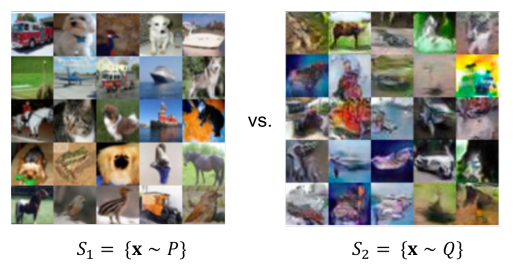
\includegraphics[height=0.58\textheight, width=\textwidth, keepaspectratio]{images/gan/gan_two_dist.png}
\end{figure}

% Place this at the bottom of the frame, before \end{frame}
% \vspace{0.5em}
\begin{minipage}{\textwidth}
\footnotetext{GANs aim to replicate data distributions, but we rarely have access to
the true probability distribution function. Instead, we compare samples
from the real data distribution with those generated by the model.}
\end{minipage}

\framebreak

\begin{itemize}
    \item Let's consider a test statistic $T$ for this purpose.
    \item Test statistic $T$ compares $S_1$ and $S_2$ e.g., difference in means, variances of the two sets of samples.
    \item \textbf{Key observation}: Test statistic is likelihood-free since it does not involve the densities $P$ or $Q$ (only samples)
\end{itemize}
\end{frame}
\begin{frame}{}
    \LARGE GANs: \textbf{Definition and Core Components}
\end{frame}

\begin{frame}{Definition and Core Components}
\begin{itemize}
    \item Let $S_1 = D = \{x \sim p_{\text{data}}\}$ and $S_2 = \{x \sim p_\theta\}$.
    \item \textbf{Idea}: Train the generative model to minimize a two-sample test objective between $S_1$ and $S_2$, i.e., the generator.
    \item<2-> \textbf{Question}: How do we obtain a two-sample test objective?
    \item<3-> \textbf{Another Idea}: Train another neural network to discriminate between the two samples, i.e., the discriminator.
    \item<4-> And Voila! That's how we arrive at a GAN. The remaining step is to define the training method.
\end{itemize}
\end{frame}

\begin{frame}[allowframebreaks]{GANs: Definition and Core Components}
\begin{figure}
    \centering
    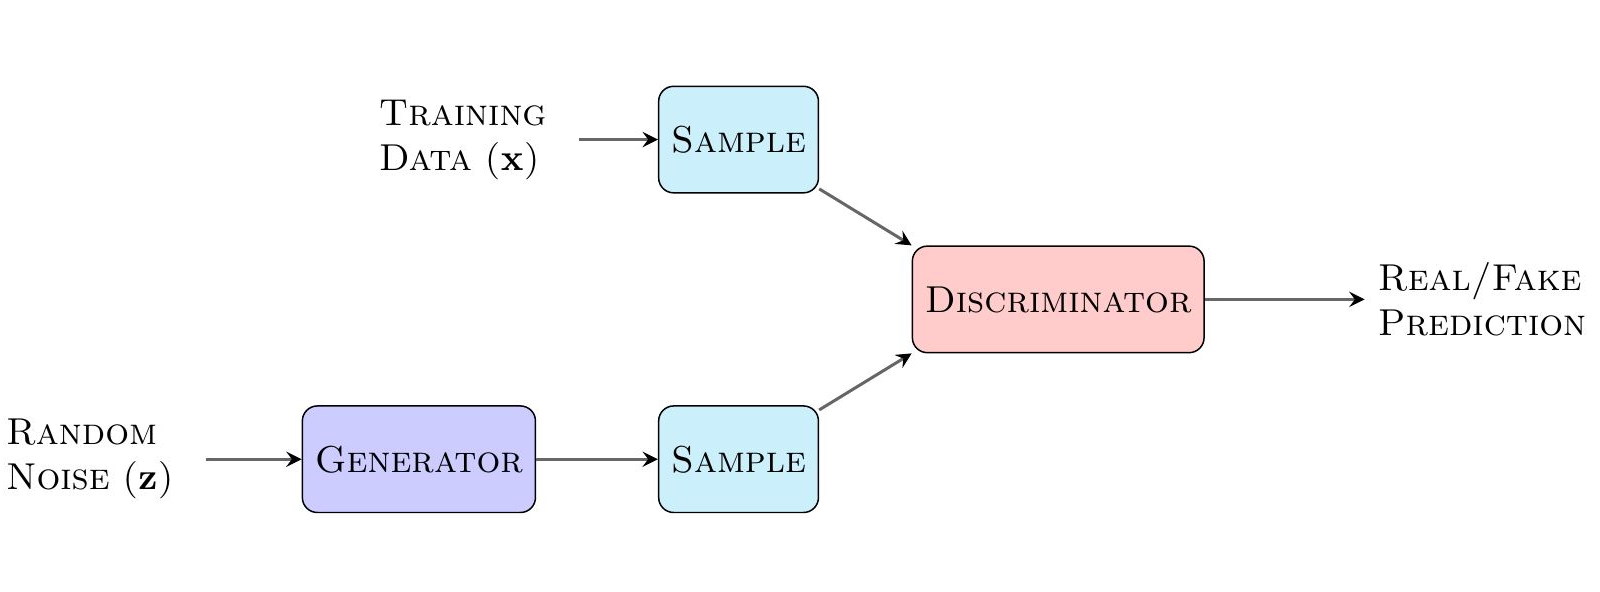
\includegraphics[height=0.7\textheight, width=\textwidth, keepaspectratio]{images/gan/gan_1.png}
    \caption*{A GAN model diagram\footnote{https://github.com/JamesAllingham/LaTeX-TikZ-Diagrams}}
\end{figure}

\framebreak

\begin{itemize}
    \item Generative Adversarial Networks were introduced by Ian Goodfellow et al. (2014).
    \item The idea behind GANs is to train two networks jointly:
    \begin{itemize}
        \item A \textbf{discriminator (D)} to classify samples as “real” or “fake”.
        \item A \textbf{generator (G)} to map a simple fixed distribution to samples that fool \textbf{D}.
    \end{itemize}
    \item The approach is \textbf{adversarial} since the two networks have opposing objectives.
\end{itemize}

\framebreak
\begin{figure}
    \centering
    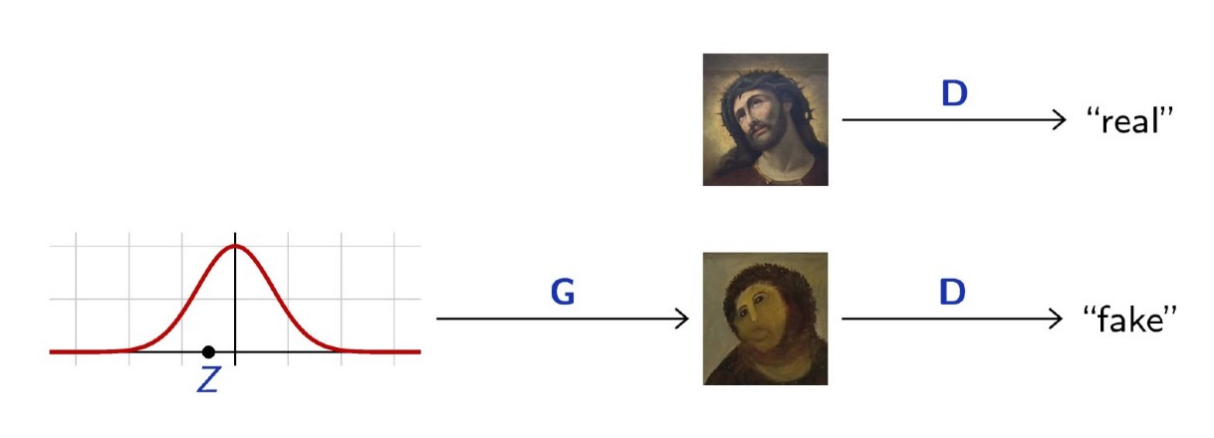
\includegraphics[height=0.7\textheight, width=\textwidth, keepaspectratio]{images/gan/gan_2.png}
    \caption*{The generator transforms a simple distribution into samples resembling real data. The discriminator distinguishes between real and fake samples.}
\end{figure}
\end{frame}
\section{Training}
\begin{frame}{}
    \LARGE GANs: \textbf{Training}
\end{frame}

\begin{frame}[allowframebreaks]{Training}
\begin{itemize}
    \item Both Discriminator and Generator are trained jointly in a min-max game.
    \item Minimax objective function:
    $$\min_{\theta_G} \max_{\theta_D} = E_{x \sim p_{data}} log(\underbrace{D_{\theta_D}(x)}_{\substack{\text{Discriminator}\\ \text{output for}\\ \text{real data }x}}) + E_{x \sim p(z)} log(1-\underbrace{D_{\theta_D}(G_{\theta_G}(z))}_{\substack{\text{Discriminator output}\\ \text{for generated fake}\\ \text{data } G(z)}})$$
    \item Discriminator $\theta_D$ wants to maximise objective such that $D(x)$ is close to 1 (real) and $D(G(z))$ is close to 0 (fake).
    \item Generator $\theta_G$ wants to minimise objective such that $D(G(z))$ is close to 1 (discriminator is fooled into thinking generated $G(z)$ is real).

\end{itemize}

\framebreak
\begin{figure}
    \centering
    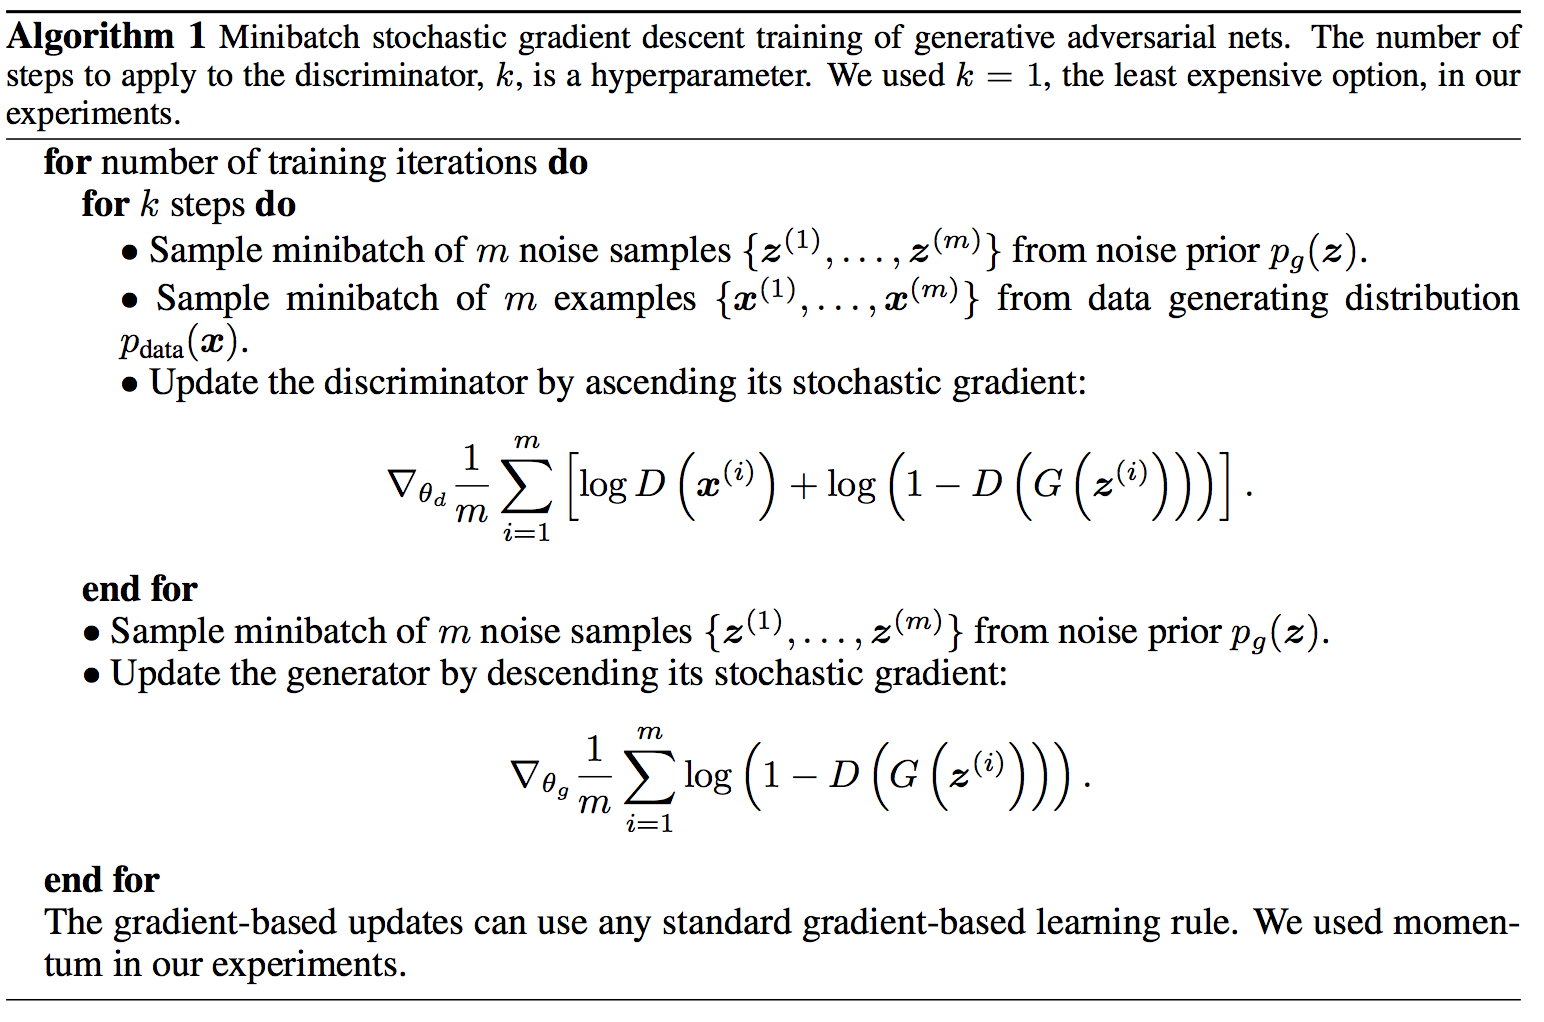
\includegraphics[height=1\textheight, width=1.02\textwidth, keepaspectratio]{images/gan/pseudocode.png}
\end{figure}

\framebreak
\textbf{The Adversarial Process:}
\begin{enumerate}
    \item Discriminator is trained to distinguish real from fake.
    \item Generator is trained to fool the discriminator.
    \item Repeat: Alternate steps until convergence.
\end{enumerate}

\textbf{Training Tips:}
\begin{itemize}
    \item Use batch normalization.
    \item Avoid sigmoid output in discriminator.
    \item Use Leaky ReLU in discriminator.
\end{itemize}

\textbf{Practical Issues:}
\begin{itemize}
    \item Discriminator becomes too strong.
    \item Gradient vanishing for generator.
    \item Careful balance of training speeds is necessary.
\end{itemize}
    
\end{frame}
\begin{frame}{}
    \LARGE GANs: \textbf{Objective function}
\end{frame}

\begin{frame}[allowframebreaks]{Understanding the Objective function}
The goal of GANs is to find a \textbf{Nash equilibrium} between the generator and discriminator. 
The generator tries to minimize the probability of the discriminator correctly classifying fake data.
\begin{figure}
    \centering
    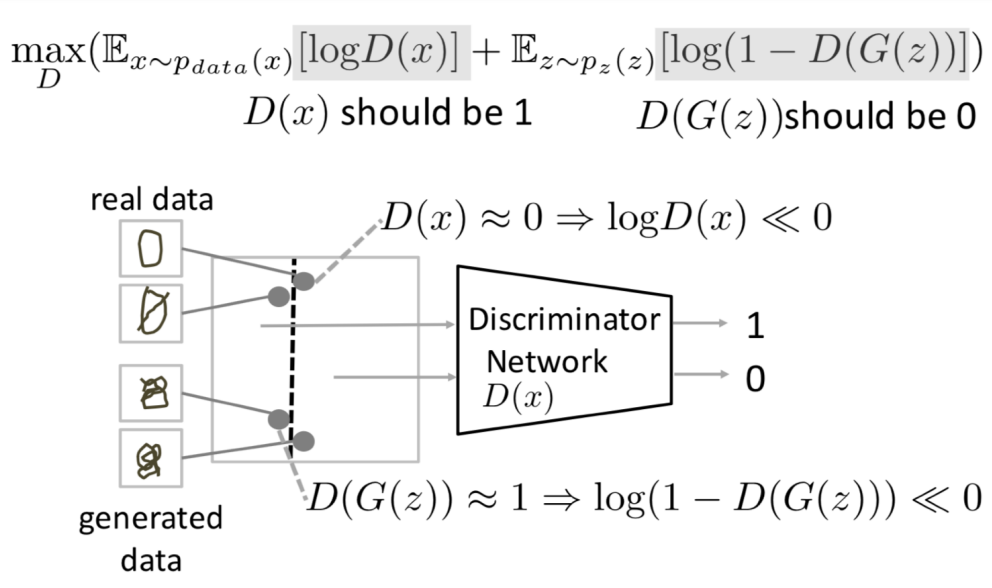
\includegraphics[height=0.7\textheight, width=\textwidth, keepaspectratio]{images/gan/gan_cost_1.png}
\end{figure}

\framebreak
\begin{figure}
    \centering
    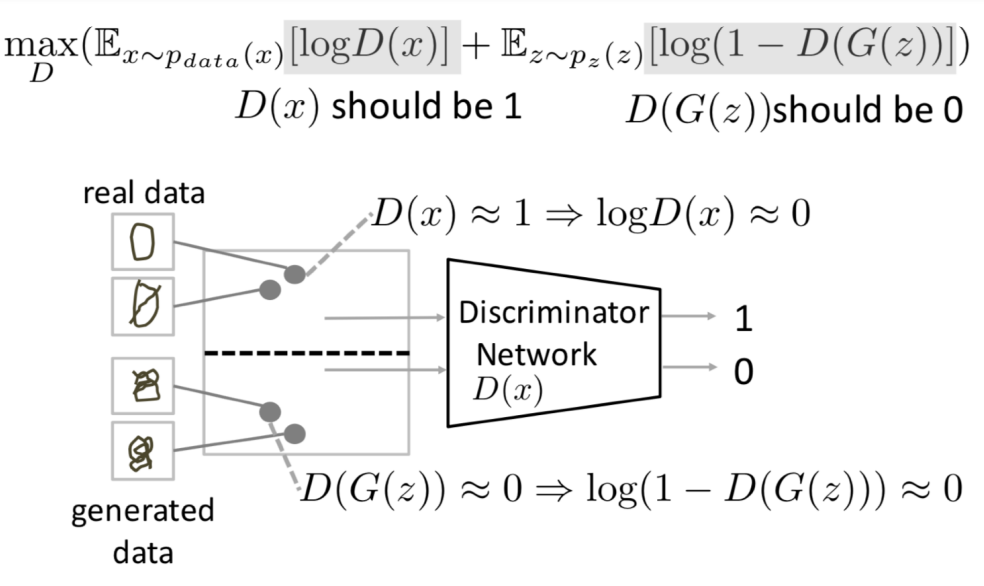
\includegraphics[height=0.9\textheight, width=\textwidth, keepaspectratio]{images/gan/gan_cost_2.png}
\end{figure}

\framebreak
\begin{figure}
    \centering
    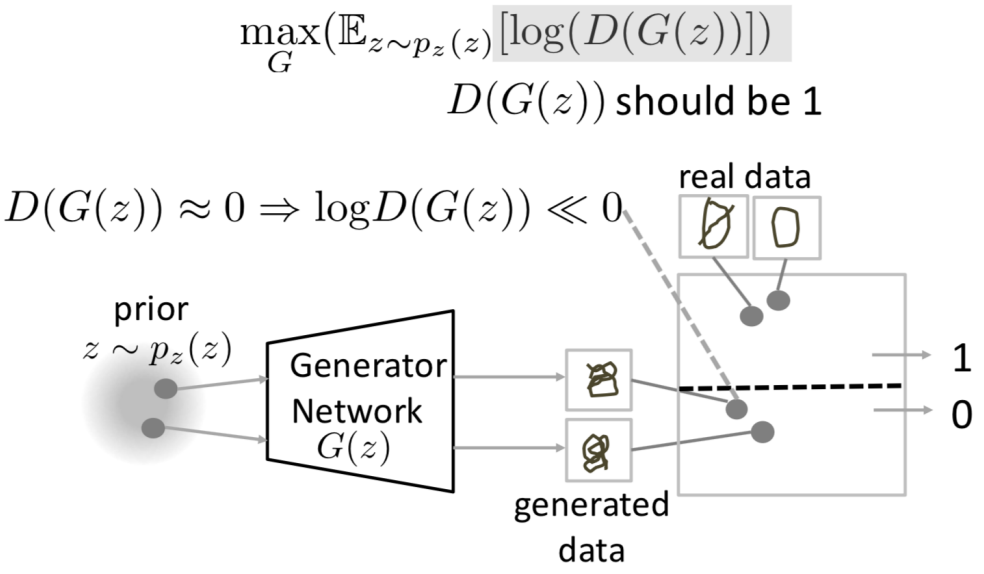
\includegraphics[height=0.9\textheight, width=\textwidth, keepaspectratio]{images/gan/gan_cost_3.png}
\end{figure}

\framebreak
\begin{figure}
    \centering
    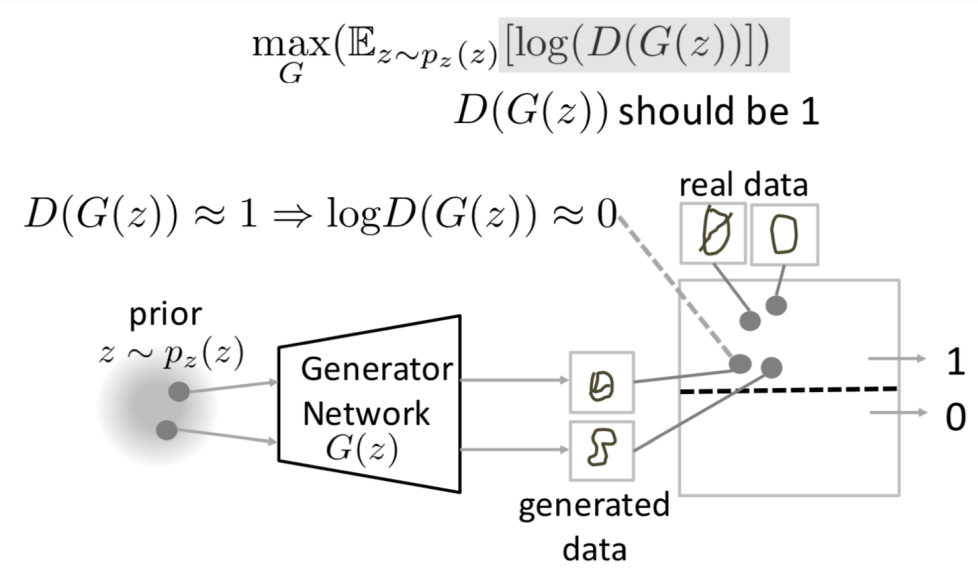
\includegraphics[height=0.9\textheight, width=\textwidth, keepaspectratio]{images/gan/gan_cost_4.png}
\end{figure}

\framebreak
\begin{figure}
    \centering
    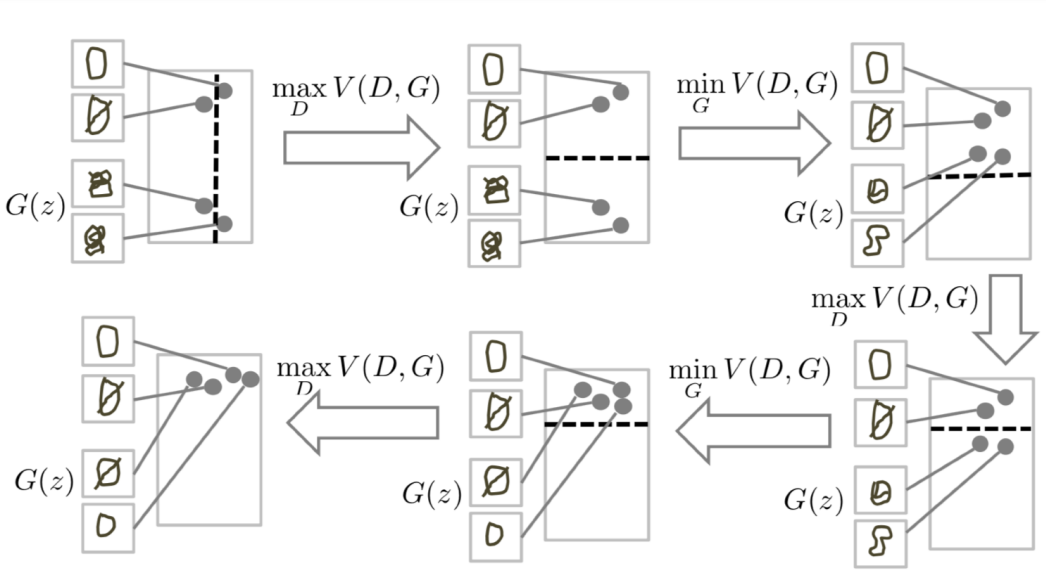
\includegraphics[height=0.9\textheight, width=\textwidth, keepaspectratio]{images/gan/gan_cost_5.png}
\end{figure}


\footnotetext{https://www.slideshare.net/ckmarkohchang/generative-adversarial-networks}
\end{frame}

\begin{frame}{GANs - Interactive Demo}
\centering
\href{https://poloclub.github.io/ganlab/}{https://poloclub.github.io/ganlab/}
    
\end{frame}
\begin{frame}{}
    \LARGE GANs: \textbf{Results}
\end{frame}

\begin{frame}[allowframebreaks]{Results}
\begin{figure}
    \centering
    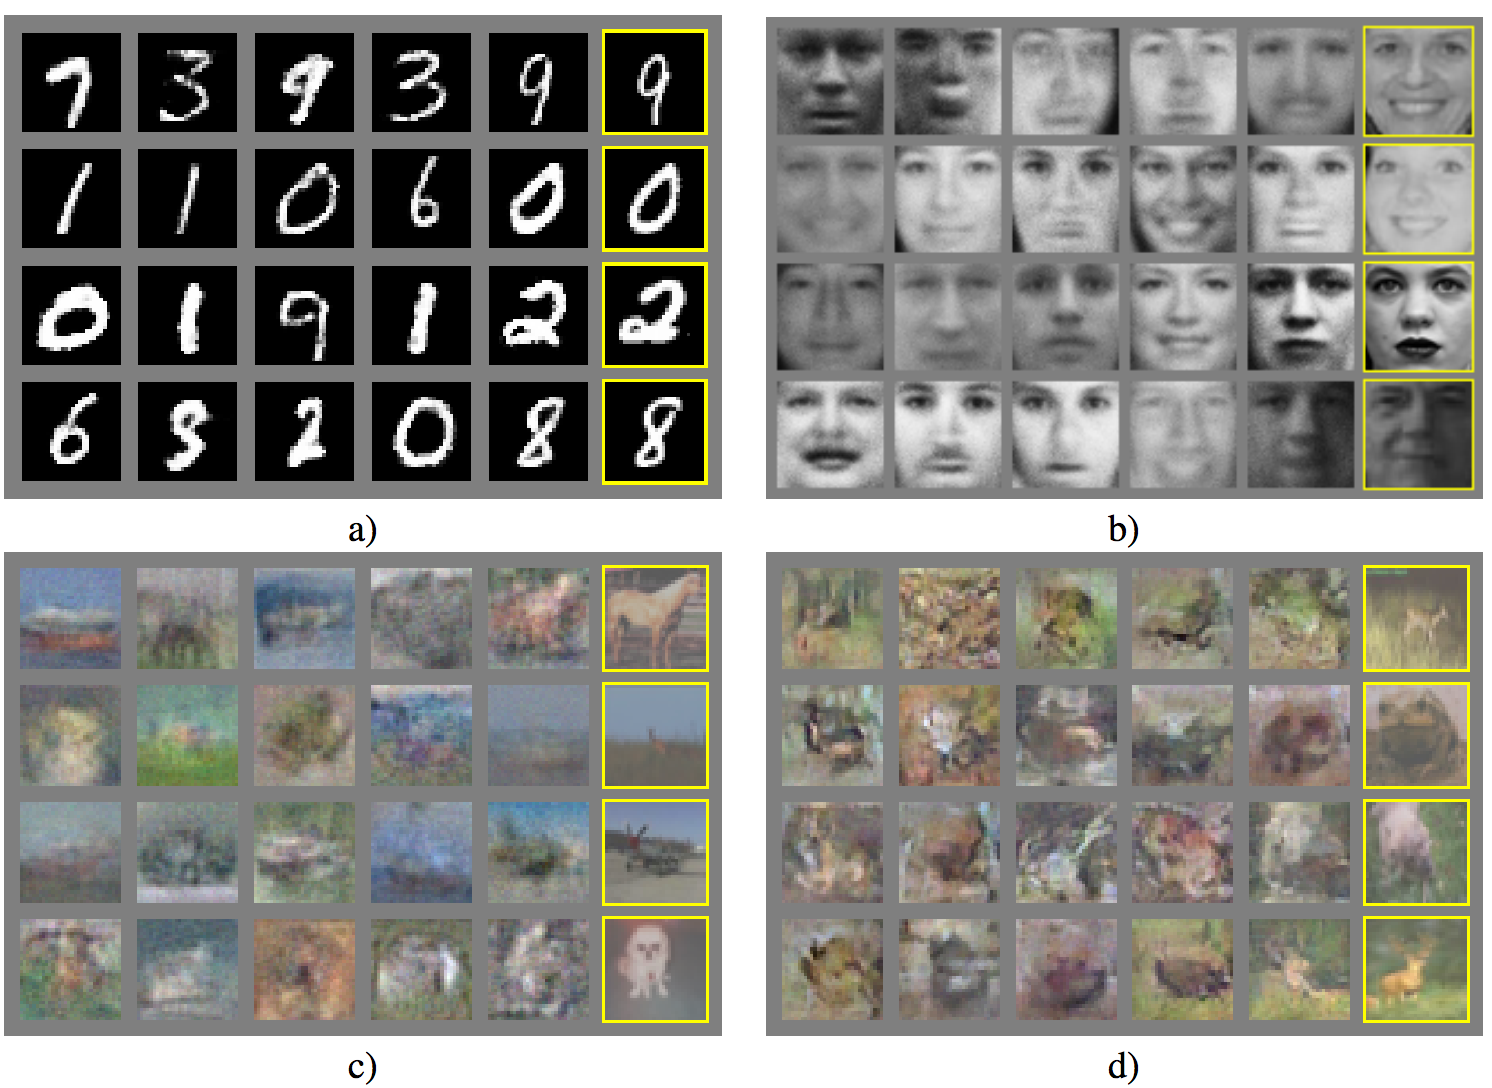
\includegraphics[height=0.8\textheight, width=\textwidth, keepaspectratio]{images/gan/result-goodfellow.png}
    \caption*{Figure from Goodfellow et al 2014, showing GAN results on various datasets.}
\end{figure}

\framebreak
\begin{figure}
    \centering
    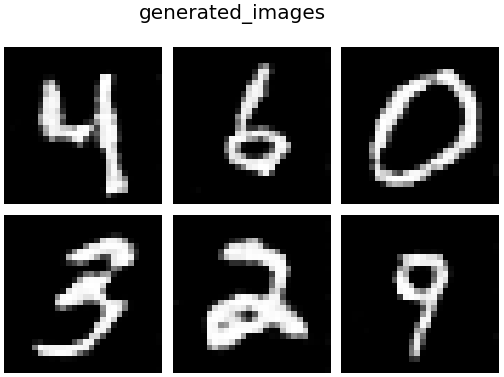
\includegraphics[height=0.8\textheight, width=\textwidth, keepaspectratio]{images/gan/gan_results_mnist.png}
    \caption*{GAN generated samples for MNIST digits dataset}
\end{figure}

\framebreak
\begin{figure}
    \centering
    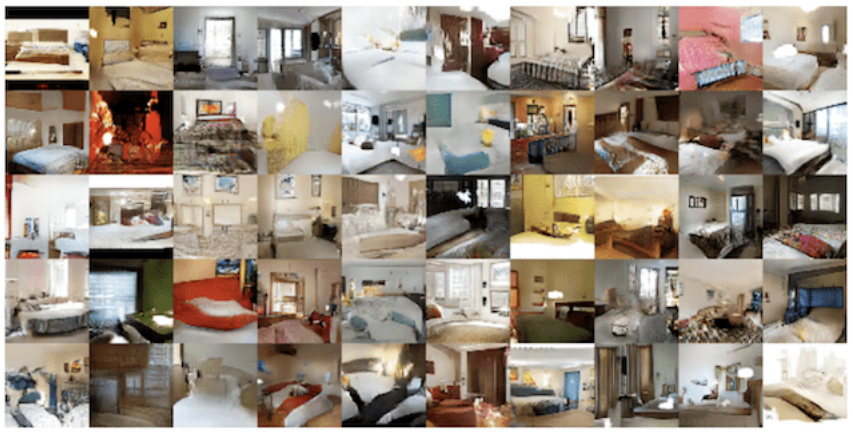
\includegraphics[height=0.8\textheight, width=\textwidth, keepaspectratio]{images/gan/gan_results_2.png}
    \caption*{GAN generated samples for bedroom images}
\end{figure}

\framebreak
\begin{figure}
    \centering
    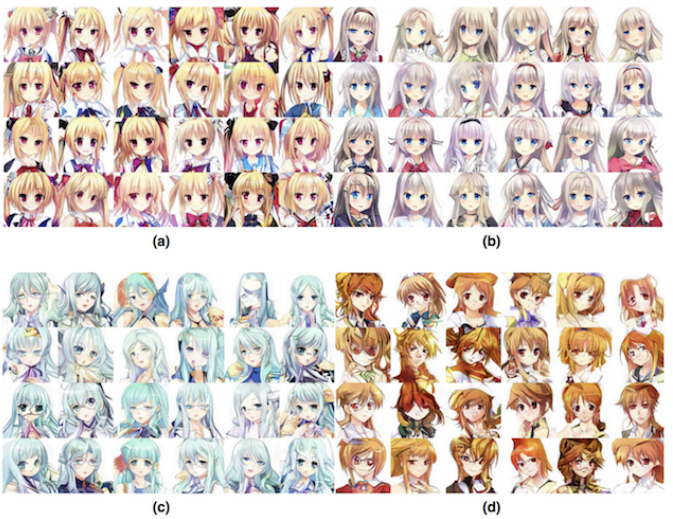
\includegraphics[height=0.8\textheight, width=\textwidth, keepaspectratio]{images/gan/gan_results_3.png}
    \caption*{GAN generated samples for anime character faces}
\end{figure}
    
\end{frame}
\section{Problems}
\begin{frame}{}
    \LARGE GANs: \textbf{Problems}
\end{frame}

\begin{frame}[allowframebreaks]{Problems with GANs}
\textbf{\large Vanishing Gradients }
    \begin{itemize}
        \item When the discriminator is perfect, we are guaranteed with $D(x) = 1, \forall x \in p_{data}$ and $D(x) = 0, \forall x \in p_G$.
        \item The loss function drops to zero, resulting in no gradient for updates.
        \item \textbf{Solution}: Perform gradient ascent on the generator, i.e., use a different objective:
        $$\max_{\theta_G} E_{x \sim p(z)} log(D_{\theta_D}(G_{\theta_G}(z)))$$
    \end{itemize}
\framebreak

\begin{figure}
    \centering
    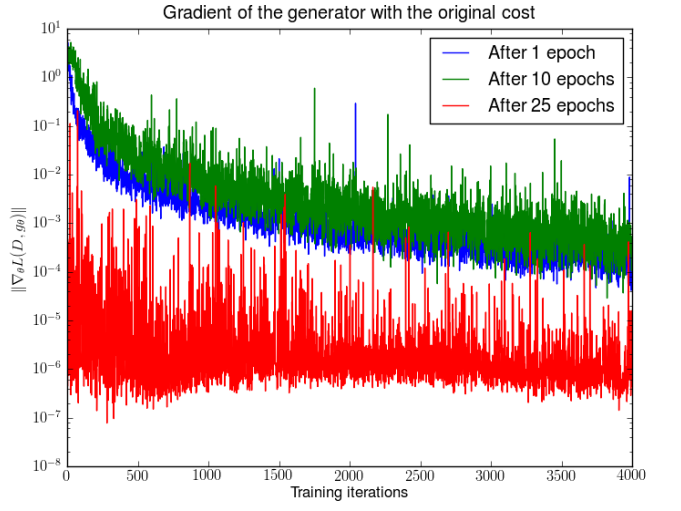
\includegraphics[height=0.8\textheight, width=\textwidth, keepaspectratio]{images/gan/gan_generator_gradient.png}
    \caption*{Vanishing gradient in GANs (Image source: \href{https://arxiv.org/pdf/1701.04862.pdf}{Arjovsky and Bottou, 2017})}
\end{figure}

\framebreak

\textbf{\large Difficulty in achieving Nash equilibrium}
    \begin{itemize}
        \item GANs involve training two models simultaneously to reach a Nash equilibrium in a two-player non-cooperative game. However, since each model updates its cost independently, convergence is not guaranteed.
        \item For practical tips on training GANs, see "How to Train a GAN? Tips and tricks to make GANs work" by Soumith Chintala: \href{https://github.com/soumith/ganhacks}{https://github.com/soumith/ganhacks}
    \end{itemize}

\framebreak
\textbf{\large Mode collapse}
    \begin{itemize}
        \item The generator aims to fool the discriminator $D$ into classifying its outputs as real. If the generator $G$ finds a single output that consistently fools $D$, it may repeatedly produce that output, leading to mode collapse.
        \item Solutions to mode collapse are mostly empirical, including alternative architectures, modified GAN losses, and additional regularization terms.
        
        \begin{figure}
            \centering
            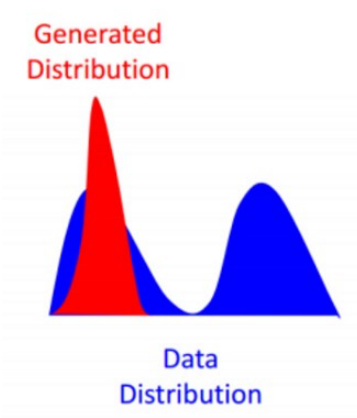
\includegraphics[height=0.4\textheight, width=\textwidth, keepaspectratio]{images/gan/gan_mode_collapse_1.png}
        \end{figure}
    \end{itemize}

\framebreak
\begin{figure}
    \centering
    
\includegraphics[height=0.85\textheight, width=\textwidth, keepaspectratio]{images/gan/gan_mode_collapse_2.png}
    \caption*{GAN mode collapse on MNIST digits dataset}
\end{figure}
    
\end{frame}
\begin{frame}{}
    \LARGE GANs: \textbf{Variants}
\end{frame}

\begin{frame}[allowframebreaks]{GAN Variants}
\begin{itemize}
    \item Since the introduction of GANs, extensive research has led to many variants.
    \item A comprehensive list of GAN variants can be found \href{https://github.com/hindupuravinash/the-gan-zoo}{here}.
\end{itemize} 
    \framebreak
    
    We will discuss the following variants:
    \begin{itemize}
        \item \textbf{Deep Convolutional GAN (DCGAN):}
        \begin{itemize}
            \item Uses convolutional and transposed convolutional layers.
            \item Employs batch normalization and ReLU/LeakyReLU activations.
            \item Improves training stability and image quality.
        \end{itemize}
        \item \textbf{Wasserstein GAN (WGAN):} 
        \begin{itemize}
            \item Introduces Wasserstein distance as the objective.
            \item Replaces sigmoid with linear output.
            \item Uses weight clipping or gradient penalty.
            \item \textbf{Variants:}
            \begin{itemize}
                \item \textbf{WGAN-GP:} Uses gradient penalty instead of weight clipping for better stability.
                \item \textbf{WGAN-LP:} Uses Lipschitz penalty as an alternative to gradient penalty.
            \end{itemize}
        \end{itemize}

\framebreak

        \item \textbf{Conditional GAN (cGAN):} 
        \begin{itemize}
            \item Conditions both the generator and discriminator on additional information (e.g., class labels).
            \item Useful for targeted generation.
        \end{itemize}
        \item \textbf{CycleGAN:} 
        \begin{itemize}
            \item Enables unpaired image-to-image translation.
            \item Uses cycle consistency loss to ensure invertibility.
        \end{itemize}
        \item \textbf{StyleGAN:} 
        \begin{itemize}
            \item Developed by NVIDIA for high-fidelity face generation.
            \item Introduces style vectors at each generator layer.
            \item Allows fine-grained control over image features.
        \end{itemize}
    \end{itemize}
\end{frame}

\subsection{Deep Convolutional GAN (DCGAN)}
\begin{frame}{}
    \LARGE GAN Variant: \\[1.5ex] \textbf{Deep Convolutional GAN (DCGAN)}
\end{frame}

\begin{frame}[allowframebreaks]{DCGAN}
    \begin{figure}
        \centering
        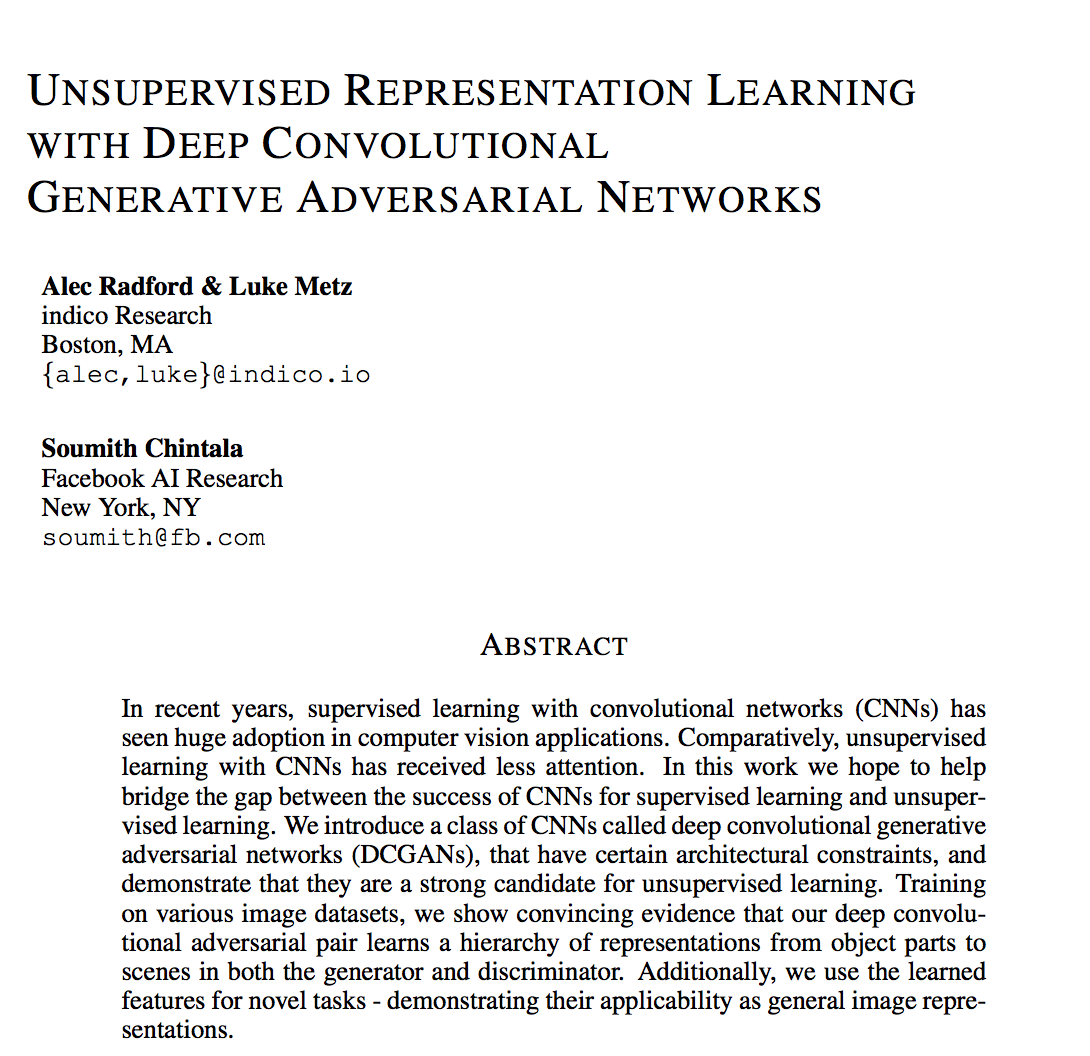
\includegraphics[height=0.9\textheight,keepaspectratio]{images/gan/dcgan-paper.png}
    \end{figure}

    \framebreak

    \begin{figure}
        \centering
        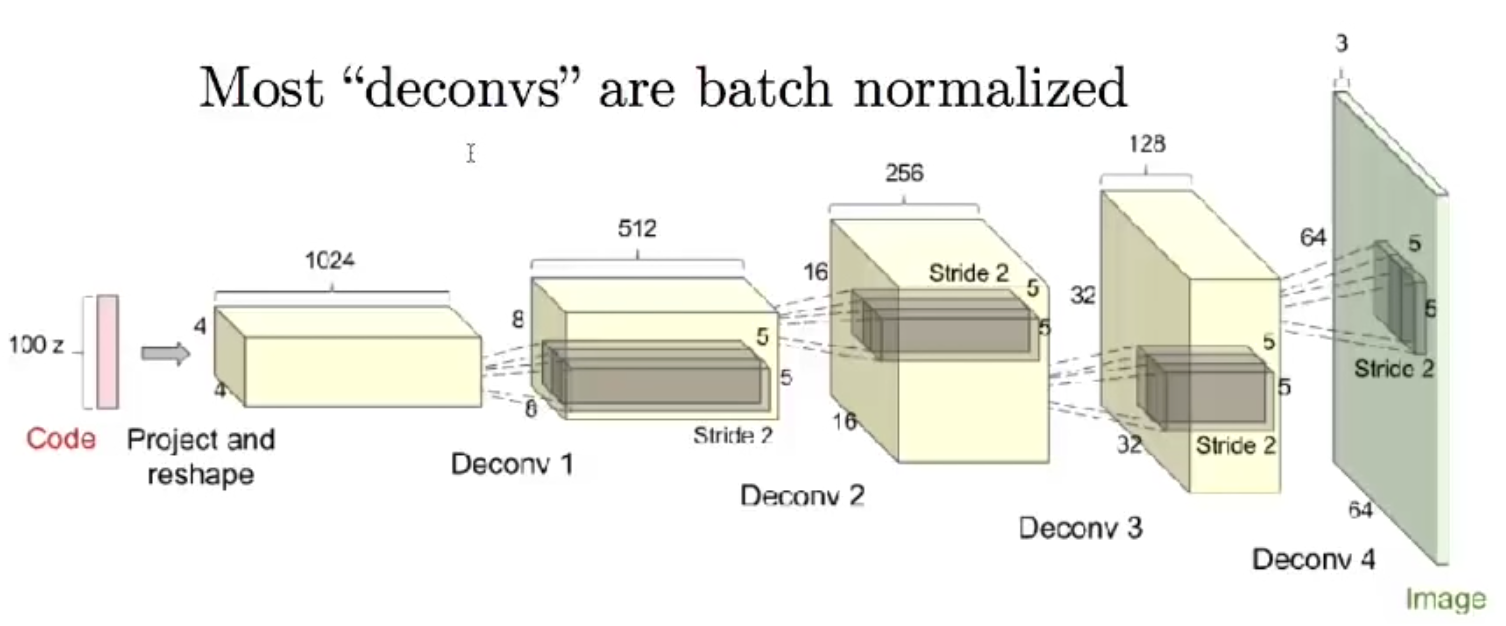
\includegraphics[width=1.05\textwidth,keepaspectratio]{images/gan/dcgan-architecture.png}
        \small [Radford et al 2016]
    \end{figure}

    \framebreak

    \textbf{Architecture Design Principles:}
    \begin{itemize}
        \item Utilizes convolutional and transposed convolutional layers instead of fully connected layers.
        \item Key architectural guidelines:
            \begin{itemize}
                \item Standard supervised CNNs are not directly usable for GANs.
                \item Remove max-pooling and mean-pooling layers.
                \item Generator upsamples using transposed convolutions.
                \item Discriminator downsamples with strided convolutions and average pooling.
                \item Non-linearity: ReLU for generator (except output), LeakyReLU (slope 0.2) for discriminator.
                \item Output non-linearity: \texttt{tanh} for generator, \texttt{sigmoid} for discriminator.
                \item Batch normalization is used to prevent mode collapse, but not applied at the output of G or input of D.
            \end{itemize}
        \item \textbf{Optimization}: Adam optimizer with learning rate $2 \times 10^{-4}$, momentum $0.5$, batch size $128$.
        \item Achieves stable training and generates high-quality images.
    \end{itemize}
\end{frame}
    
\begin{frame}[allowframebreaks]{DCGAN: Results}
    Good samples on datasets with 3M images (Faces, Bedrooms) for the first time
    \begin{figure}
        \centering
        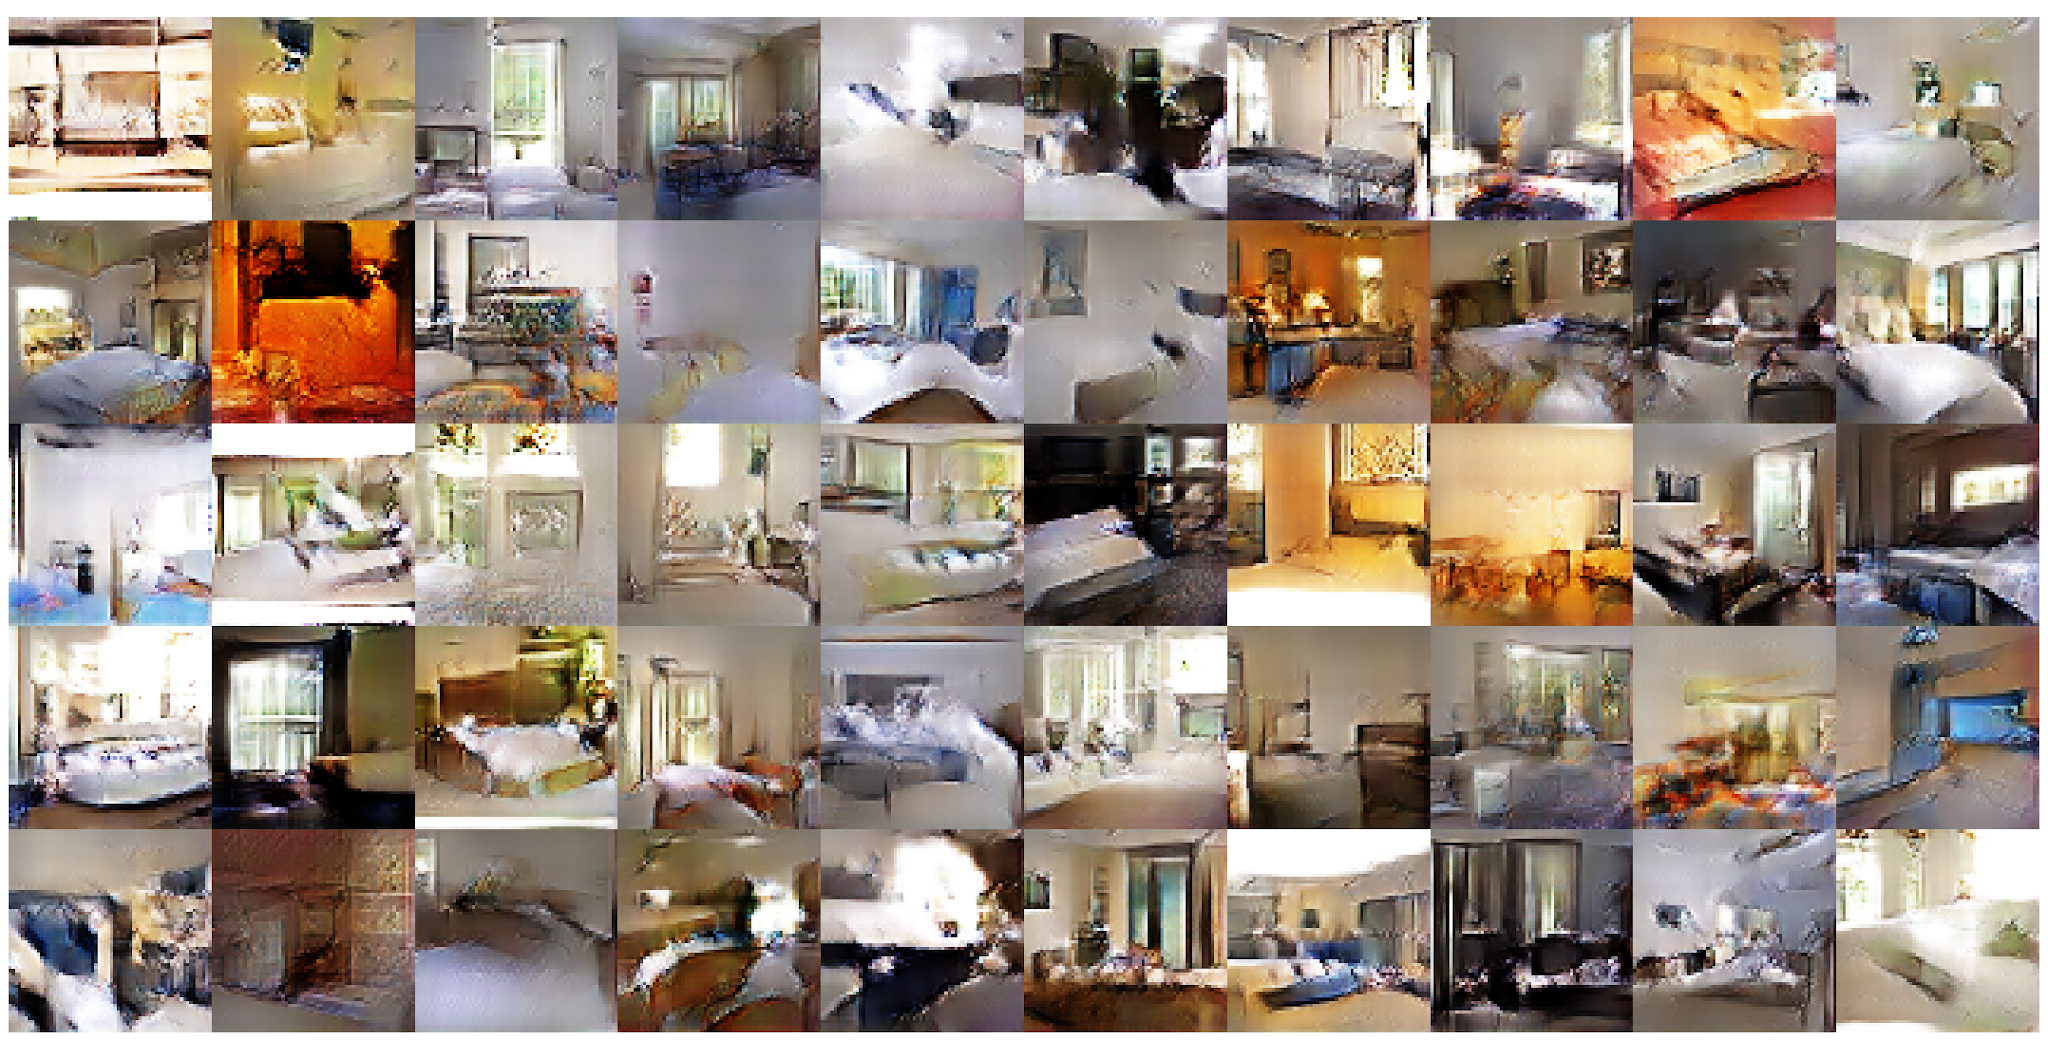
\includegraphics[width=0.9\textwidth,keepaspectratio]{images/gan/dcgan-result-1.png}
    \end{figure}
    \footnotesize{Reference: Radford, Metz, and Chintala, "Unsupervised Representation Learning with Deep Convolutional Generative Adversarial Networks", ICLR 2016}

    \framebreak

    \begin{figure}
        \centering
        \includegraphics[height=0.8\textheight,keepaspectratio]{images/gan/dcgan-result-2.png}
        \caption*{[Radford et al 2016]} 
    \end{figure}

    \framebreak

    Smooth interpolations in high dimensions
    \begin{figure}
        \centering
        \includegraphics[height=0.8\textheight,keepaspectratio]{images/gan/dcgan-result-3.png}
        \caption*{[Radford et al 2016]}
    \end{figure}

    \framebreak

    Imagenet samples (32x32)
    \begin{figure}
        \centering
        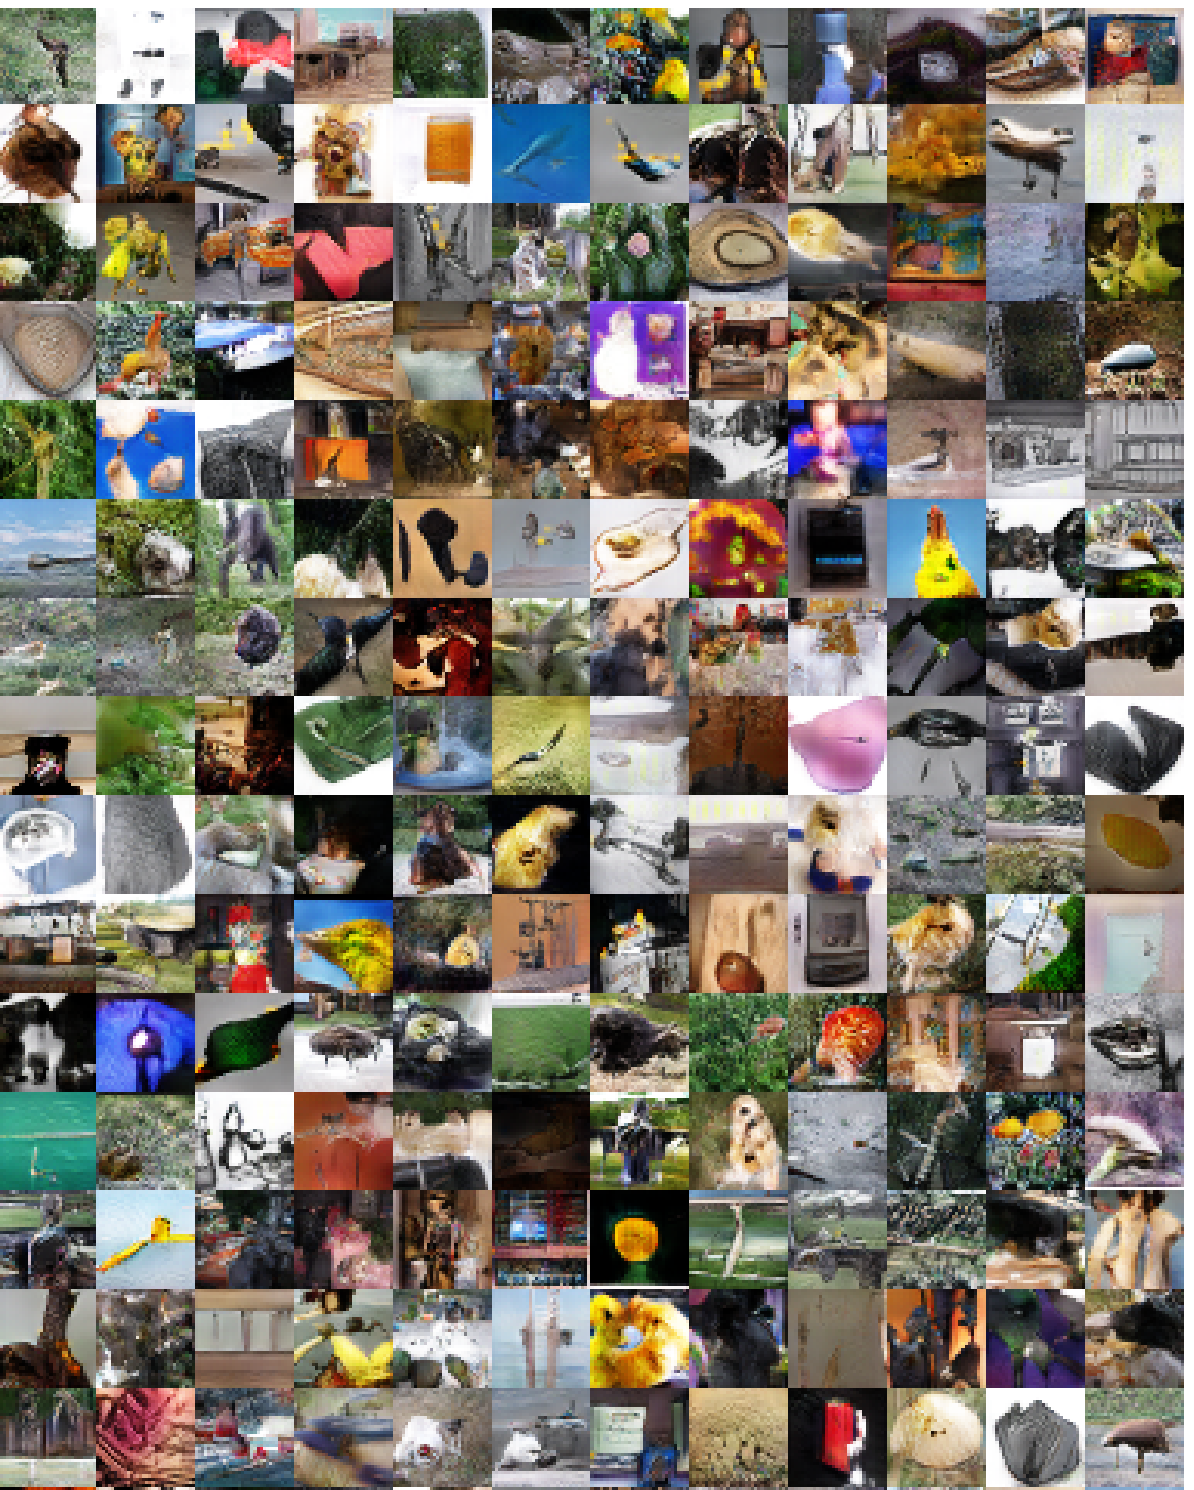
\includegraphics[height=0.8\textheight,keepaspectratio]{images/gan/dcgan-result-4.png}
        \caption*{[Radford et al 2016]}
    \end{figure}

    \framebreak

    Vector Arithmetic
    \begin{figure}
        \centering
        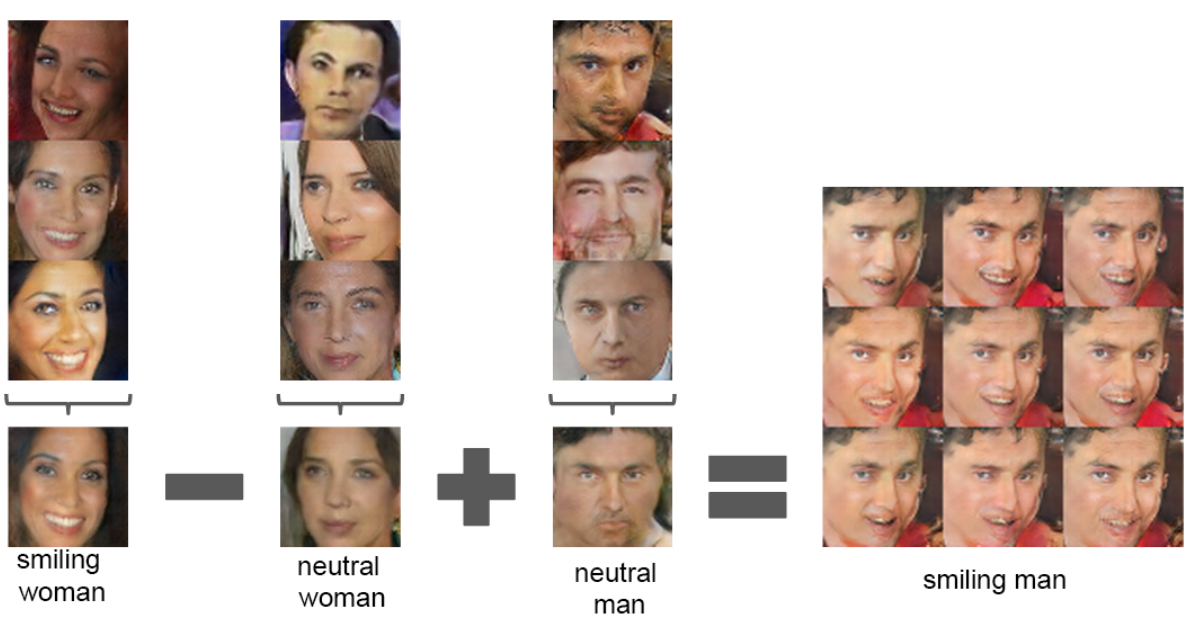
\includegraphics[height=0.75\textheight,keepaspectratio]{images/gan/dcgan-result-5.png}
        \caption*{[Radford et al 2016]}
    \end{figure}

    \framebreak

    \begin{figure}
        \centering
        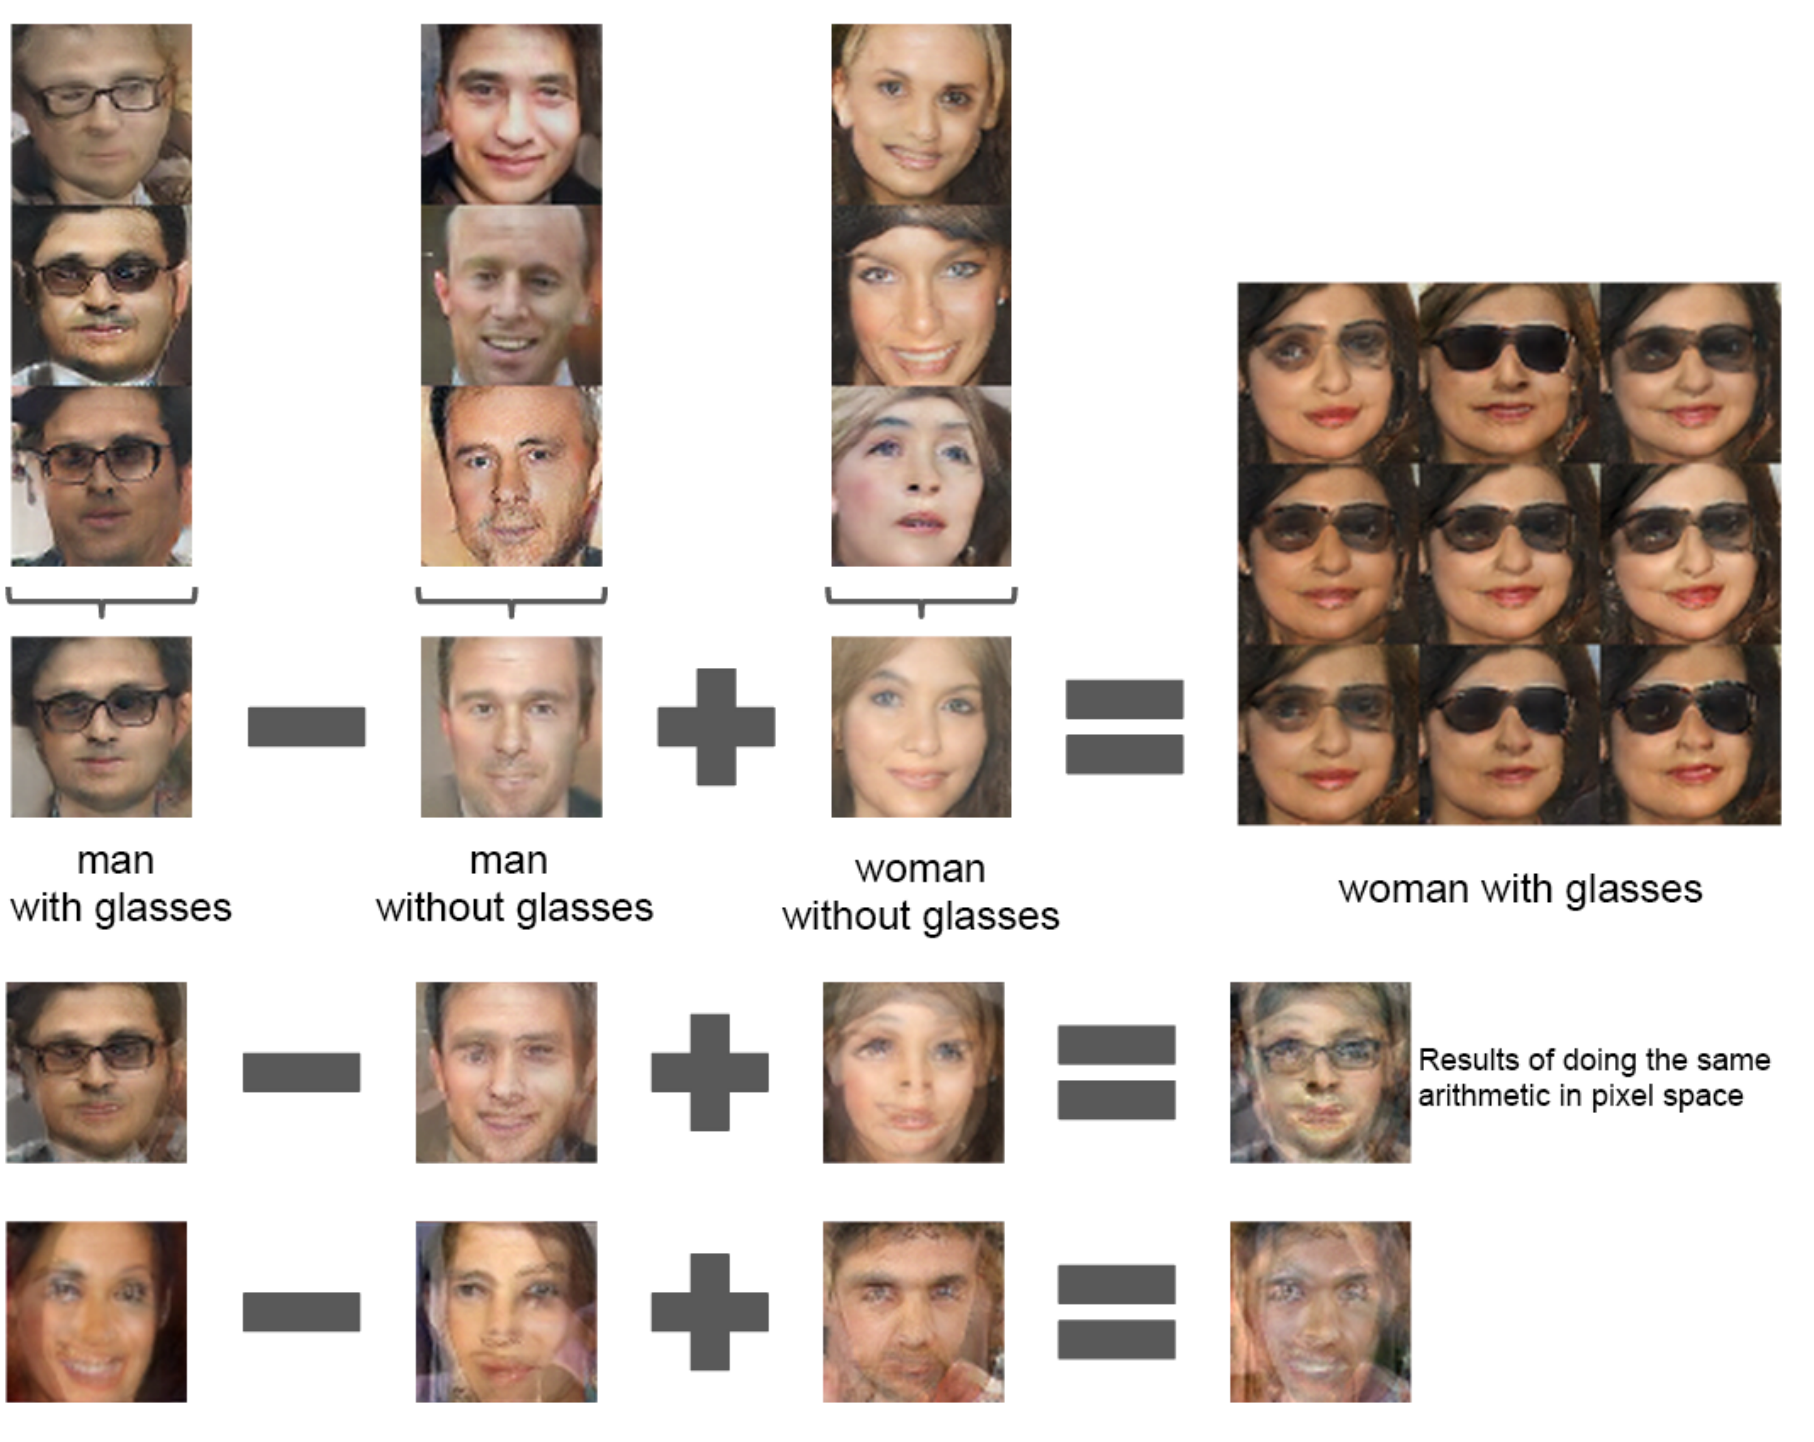
\includegraphics[height=0.8\textheight,keepaspectratio]{images/gan/dcgan-result-6.png}
        \caption*{[Radford et al 2016]}
    \end{figure}

    \framebreak

    \begin{figure}
        \centering
        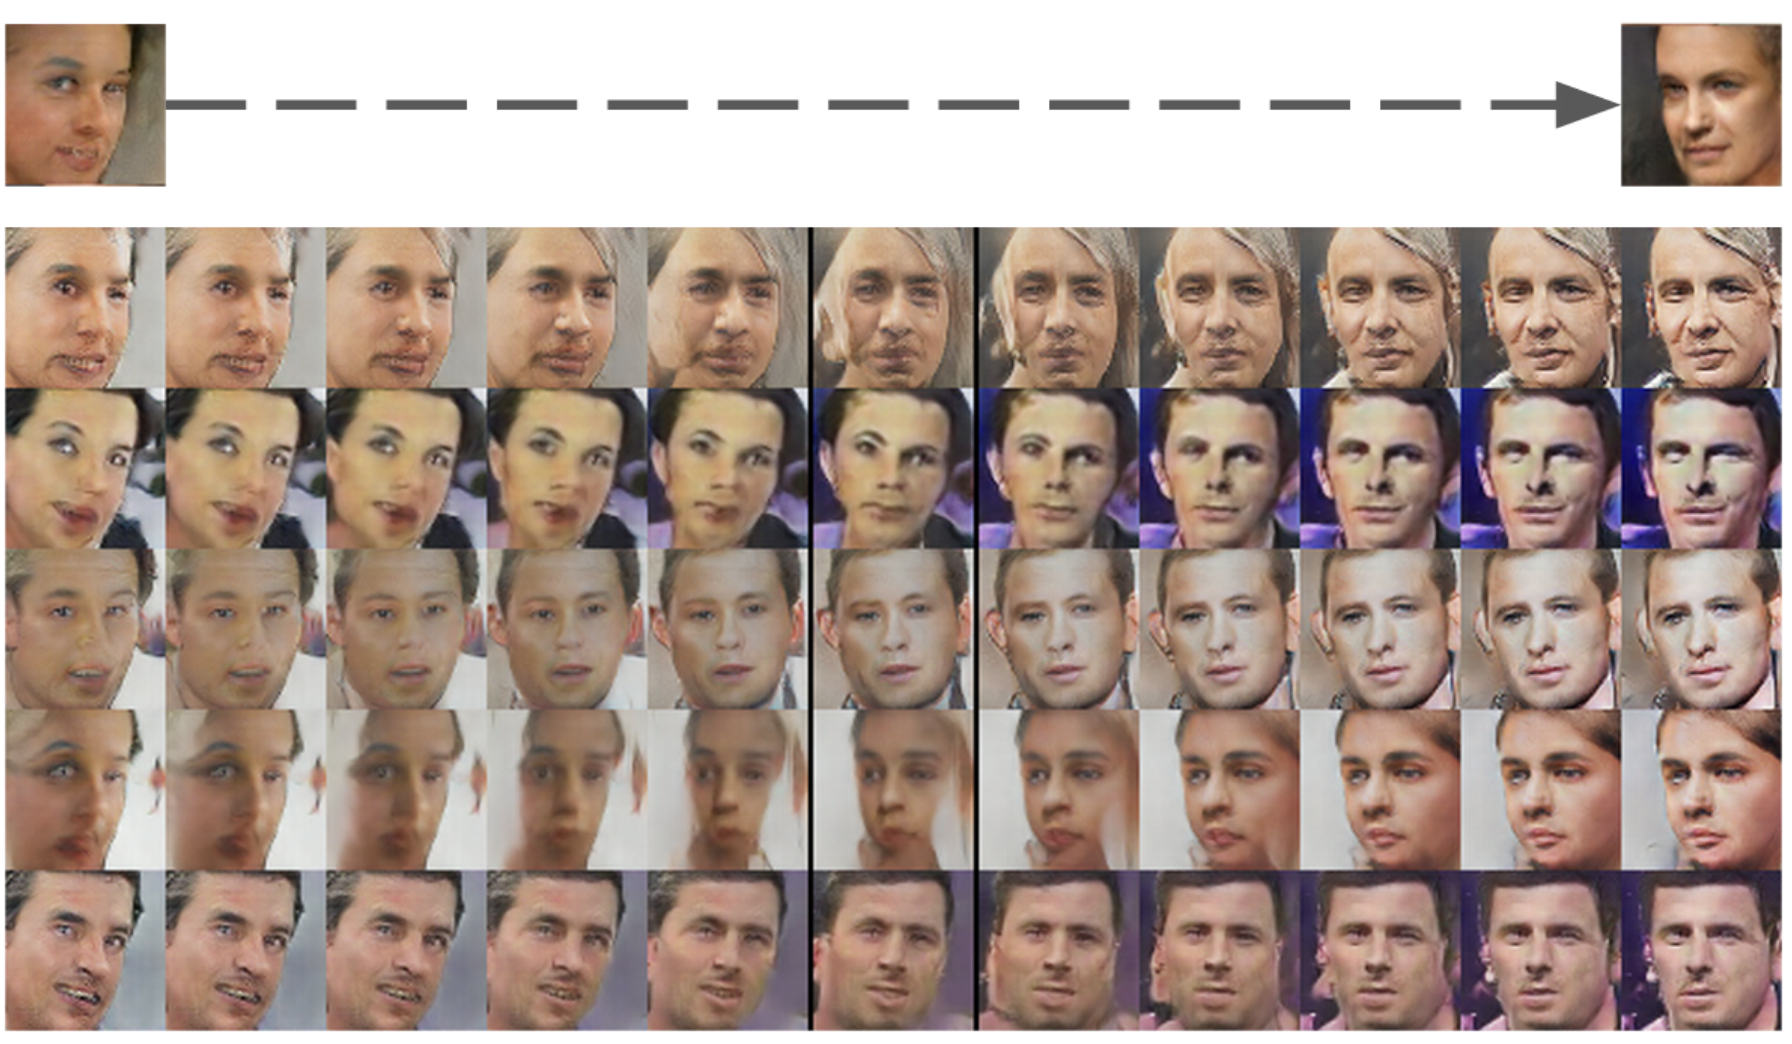
\includegraphics[height=0.8\textheight,keepaspectratio]{images/gan/dcgan-result-7.png}
        \caption*{[Radford et al 2016]}
    \end{figure}

    \framebreak

    Representation Learning 
    \begin{figure}
        \centering
        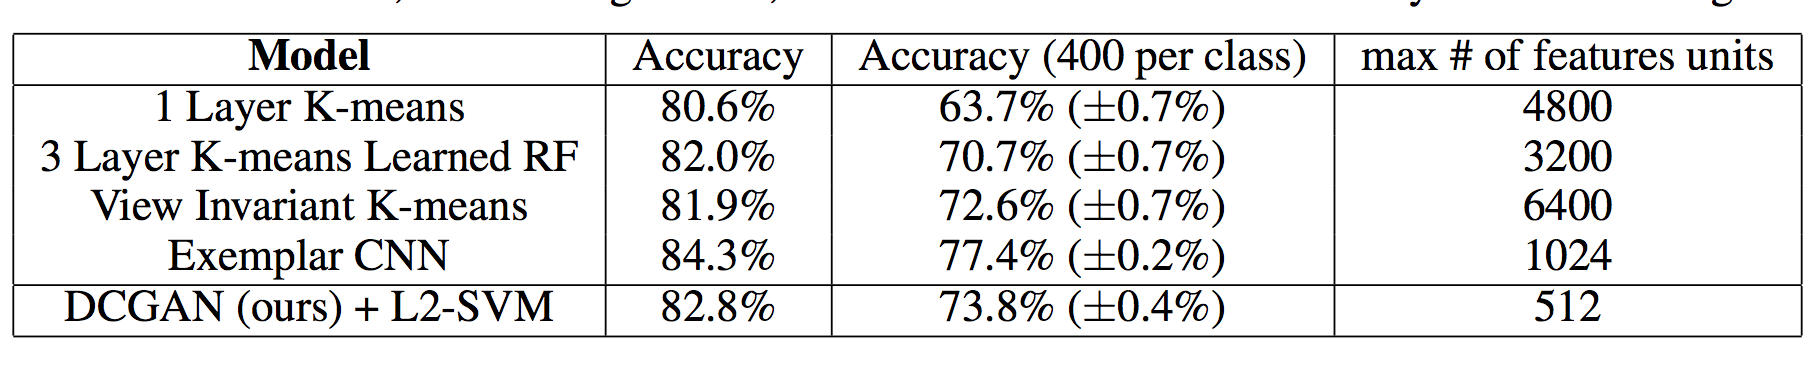
\includegraphics[width=1.05\textwidth,keepaspectratio]{images/gan/dcgan-result-table.png}
        \caption*{[Radford et al 2016]}
    \end{figure}
\end{frame}
\begin{frame}{}
    \LARGE GAN Variant: \\[1.5ex] \textbf{Wasserstein GANs (WGANs)}
\end{frame}

\begin{frame}[allowframebreaks]{Wasserstein GAN}
\begin{itemize}
    \item Wasserstein GAN uses wasserstein distance instead of crossentropy loss.
    \item Wasserstein distance that has a smoother gradient everywhere.
        \begin{figure}
            \centering
            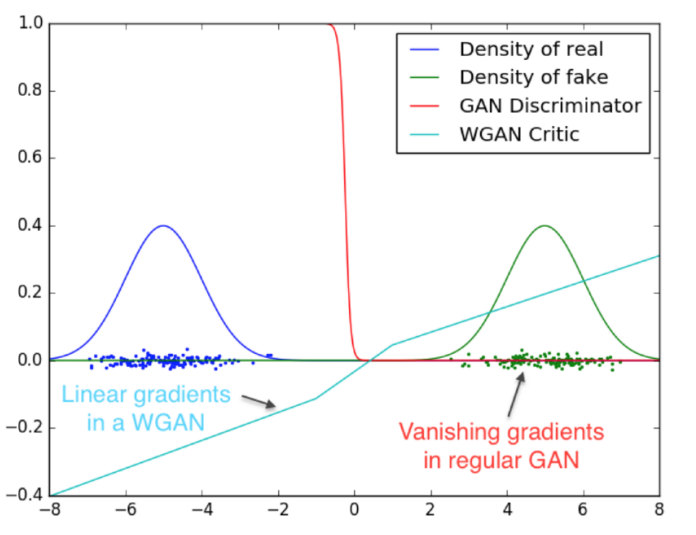
\includegraphics[height=0.6\textheight, width=\textwidth, keepaspectratio]{images/gan/wgan_1.png}
        \end{figure}
\end{itemize}
    
\end{frame}

\begin{frame}{Wasserstein Distance}
\begin{itemize}
    \item Intuitively, it is the shovels of earth moved to make two distributions look alike.
    \begin{figure}
        \centering
        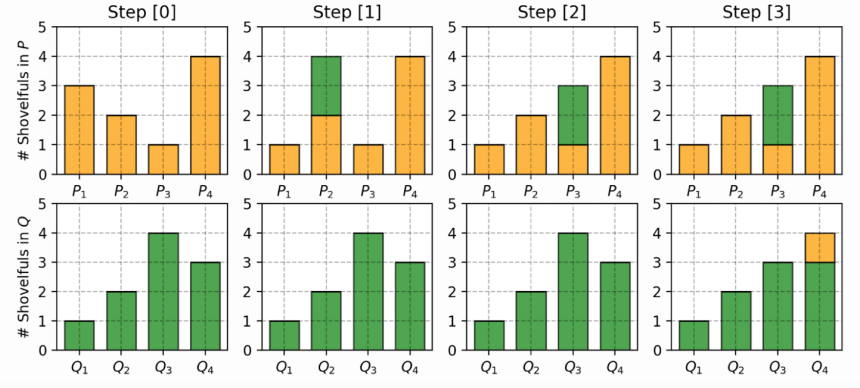
\includegraphics[height=0.6\textheight, width=\textwidth, keepaspectratio]{images/gan/wgan_2.png}
        \caption*{Step by Step plan of moving dirt between piles $P$ and $Q$ to make them match}
    \end{figure}
    
\end{itemize}
    
\end{frame}

\begin{frame}[allowframebreaks]{WGAN}
\begin{figure}
    \centering
    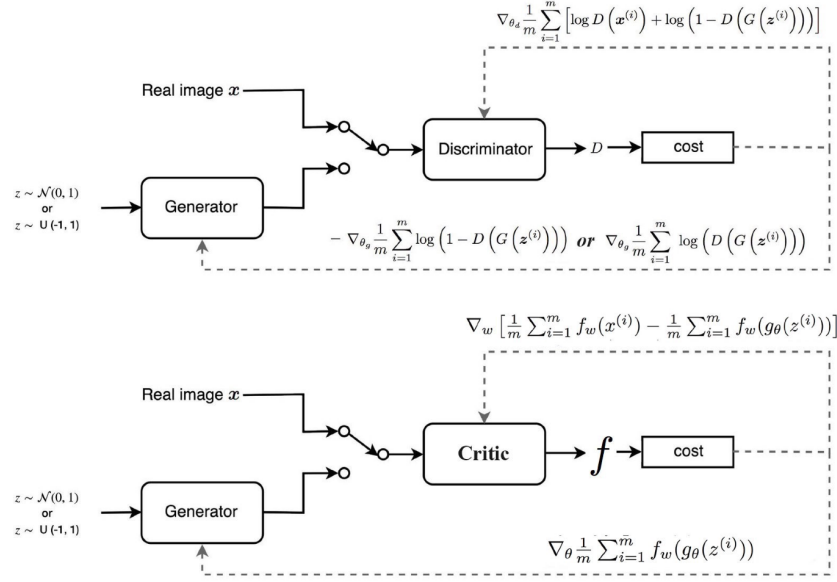
\includegraphics[height=0.9\textheight, width=\textwidth, keepaspectratio]{images/gan/wgan_3.png}
\end{figure}

\framebreak
\begin{figure}
    \centering
    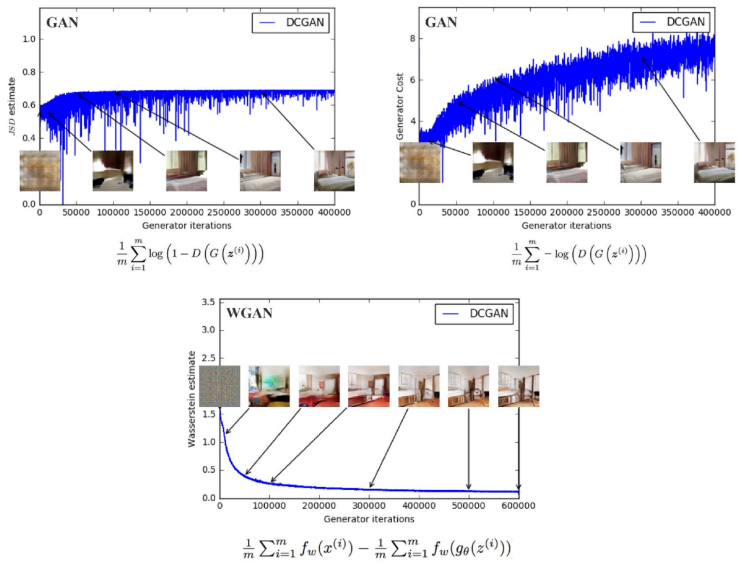
\includegraphics[height=0.9\textheight, width=\textwidth, keepaspectratio]{images/gan/wgan_4.png}
\end{figure}

\framebreak
\begin{figure}
    \centering
    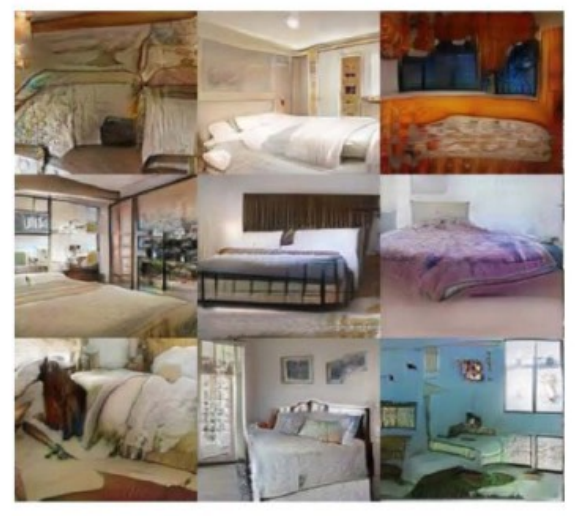
\includegraphics[height=0.8\textheight, width=\textwidth, keepaspectratio]{images/gan/wgan_5.png}
    \caption*{WGAN generation results on bedroom images}
\end{figure}

\end{frame}

\begin{frame}[allowframebreaks]{WGAN-GP: Gradient Penalty for Lipschitzness}
\begin{figure}
    \centering
    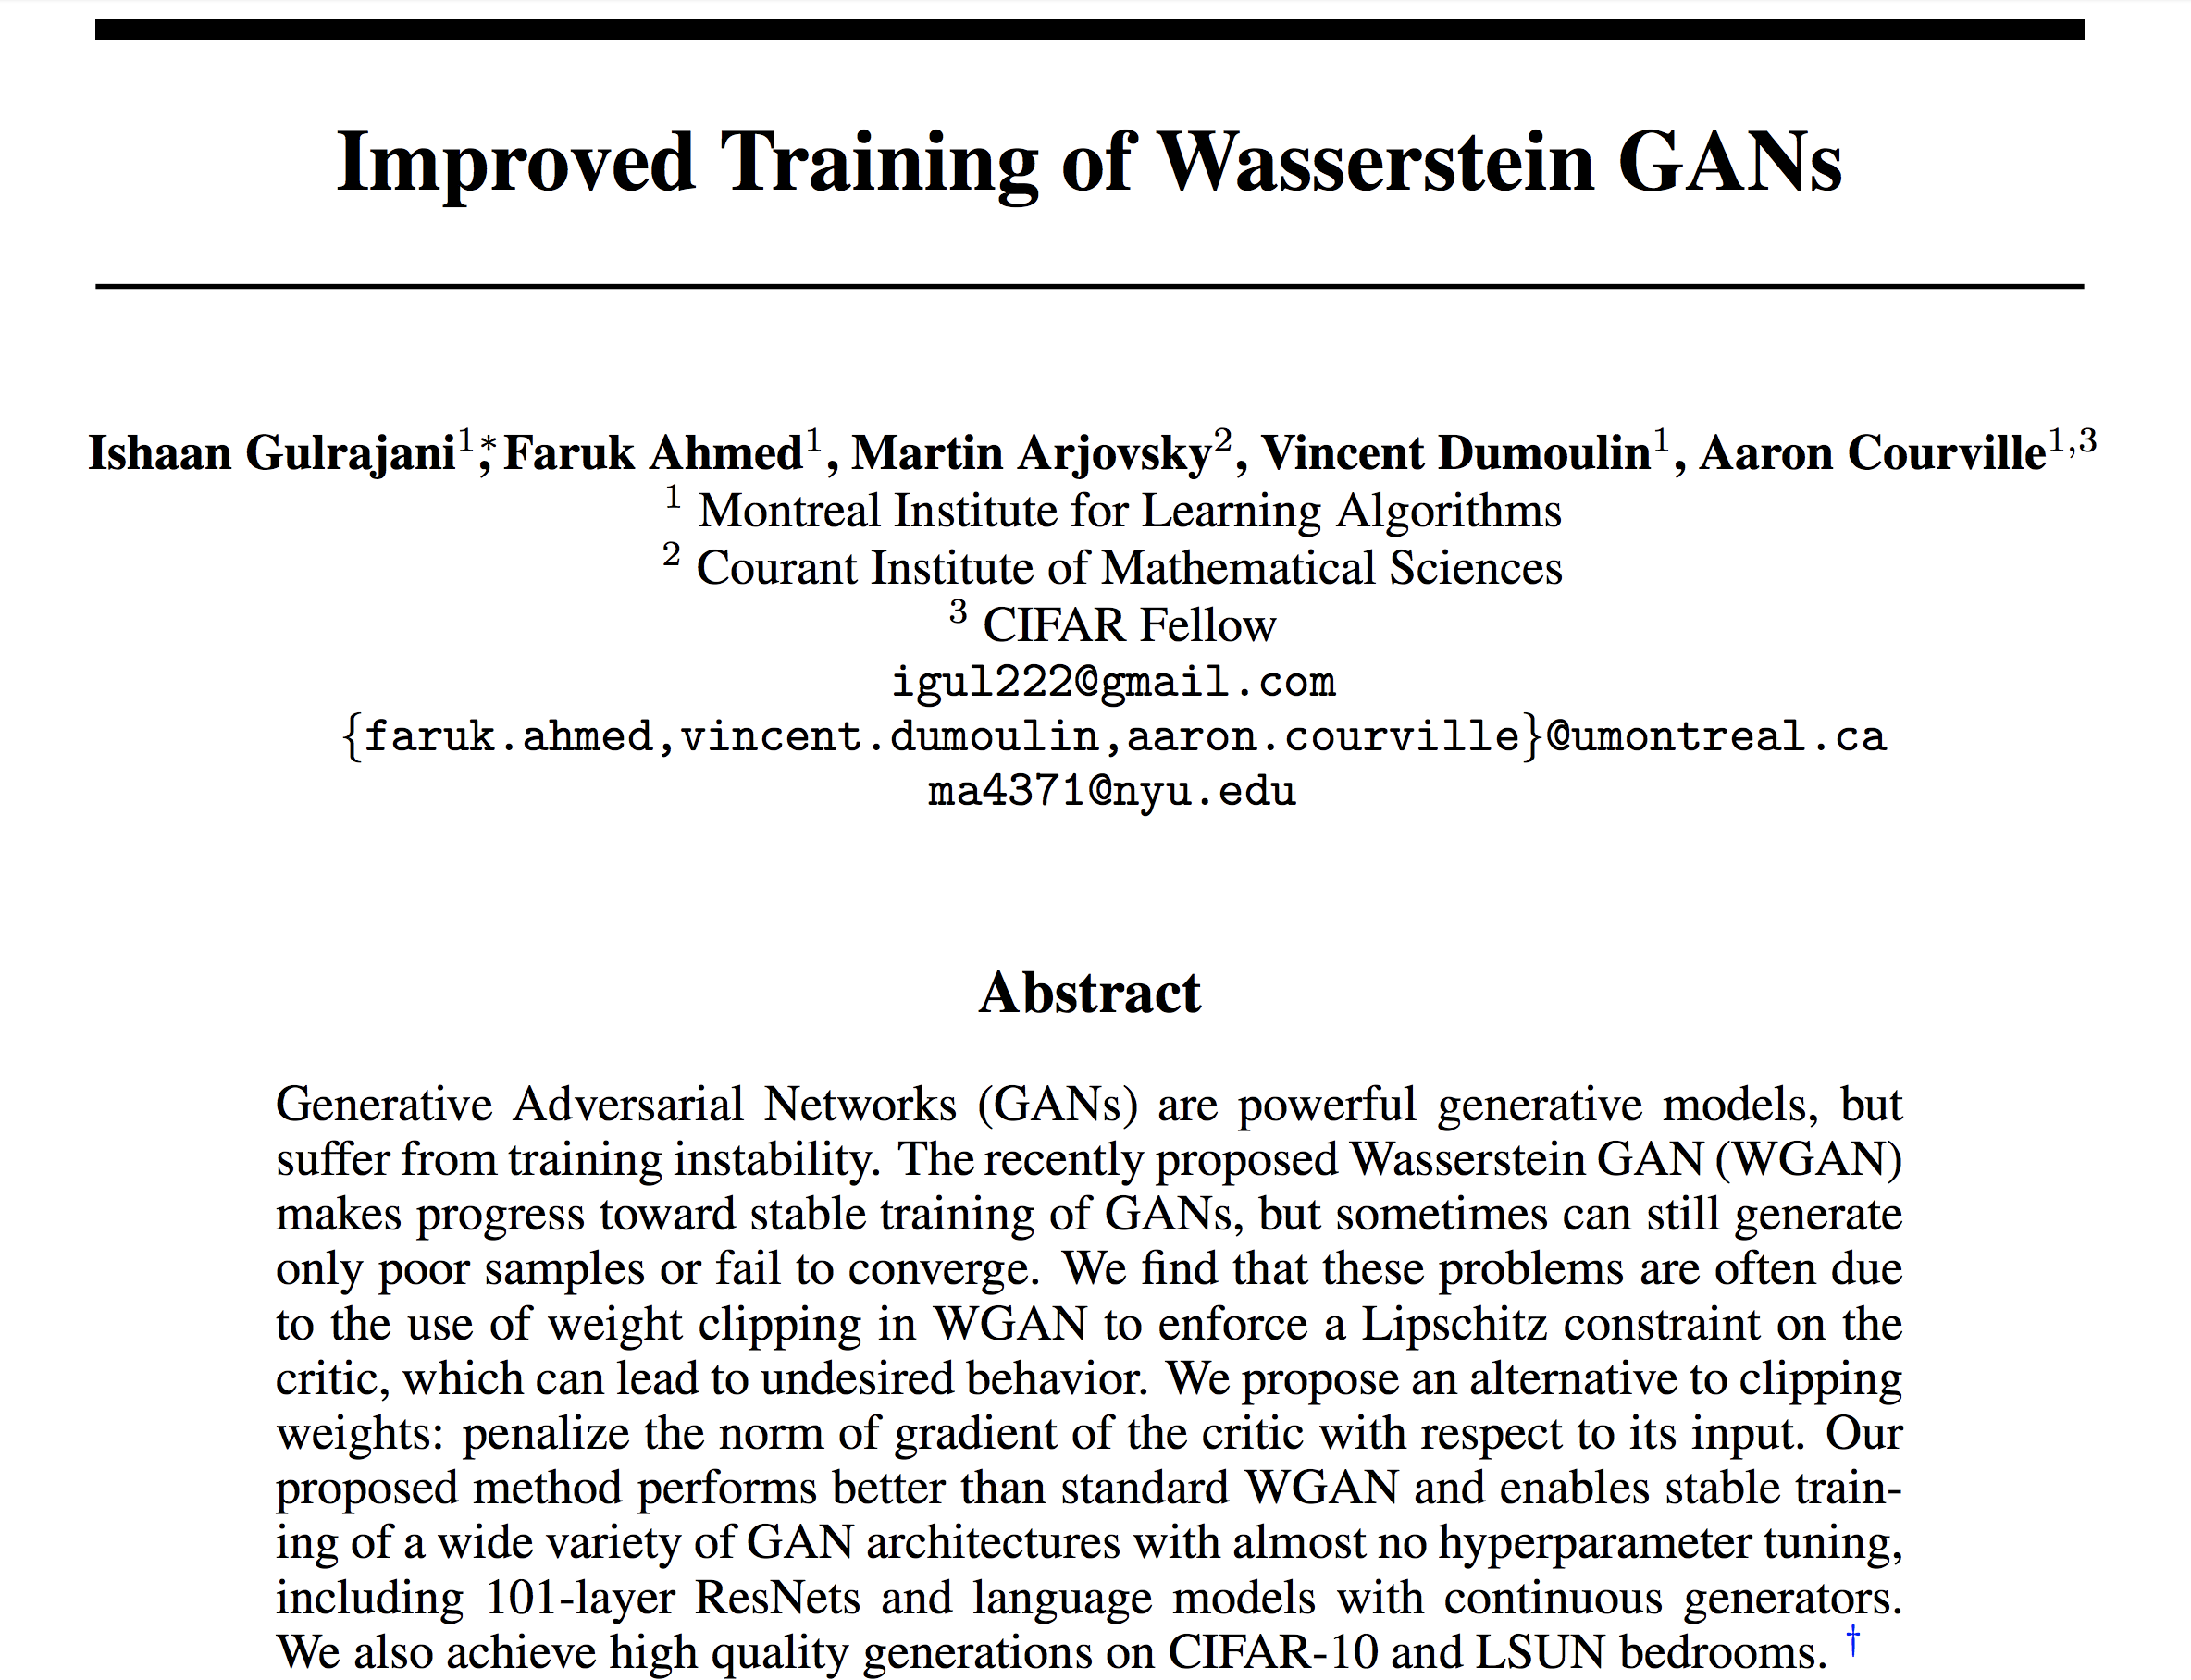
\includegraphics[height=0.8\textheight, width=\textwidth, keepaspectratio]{images/gan/wgan-gp/slide_84_1_img.png}
    \caption*{[Gulrajani et al 2017]}
\end{figure}

\framebreak
\begin{columns}
    \column{0.6\textwidth}
    \begin{figure}
        \centering
        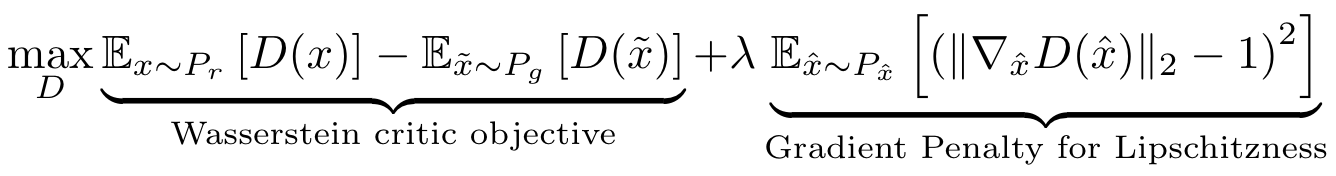
\includegraphics[height=0.8\textheight, width=\textwidth, keepaspectratio]{images/gan/wgan-gp/slide_85_3_img.png}
    \end{figure}
    \begin{figure}
        \centering
        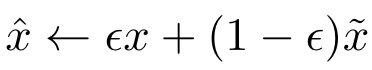
\includegraphics[height=0.1\textheight, width=\textwidth, keepaspectratio]{images/gan/wgan-gp/slide_85_4_img.png}
    \end{figure}
    \column{0.5\textwidth}
    \begin{figure}
        \centering
        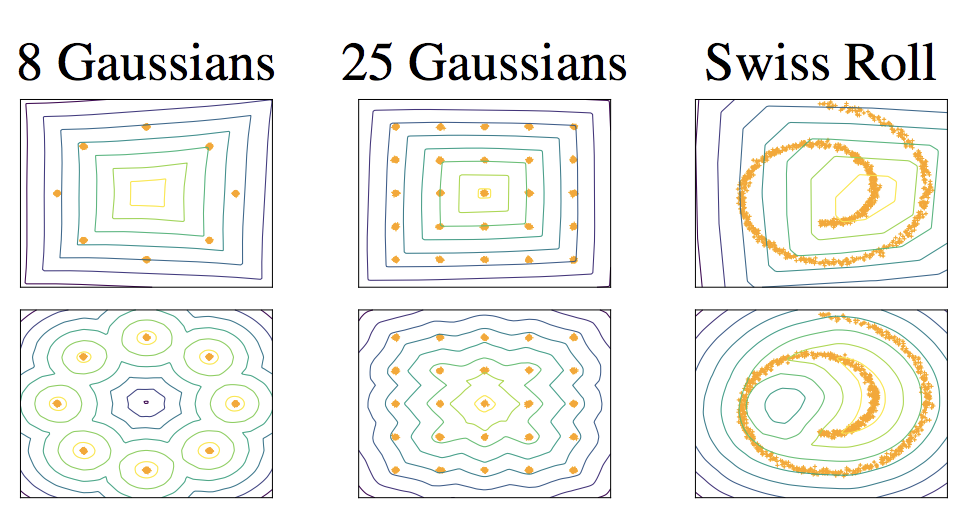
\includegraphics[height=0.8\textheight, width=1.05\textwidth, keepaspectratio]{images/gan/wgan-gp/slide_85_2_img.png}
    \end{figure}
    \begin{figure}
        \centering
        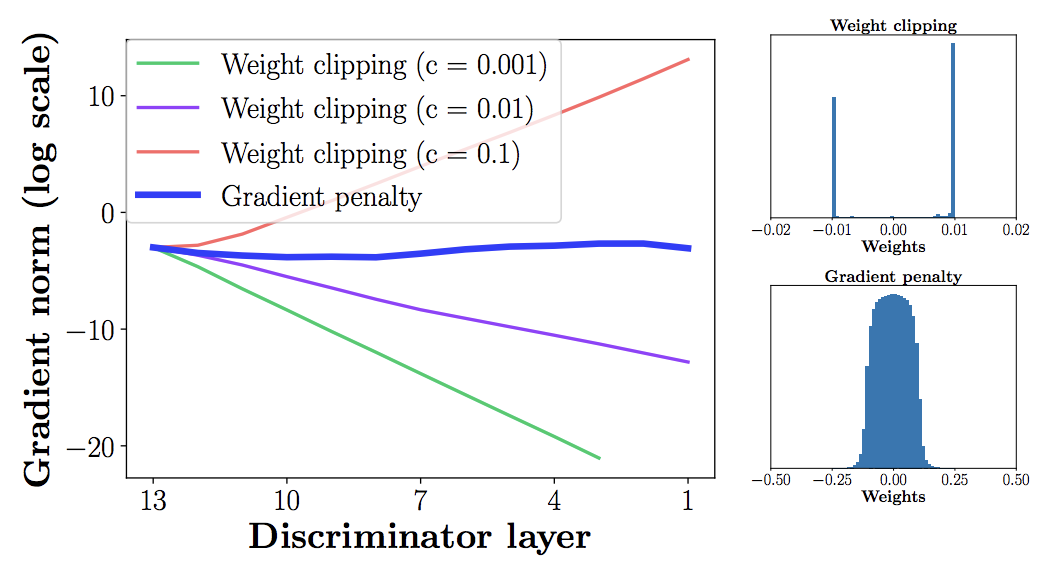
\includegraphics[height=0.8\textheight, width=1.05\textwidth, keepaspectratio]{images/gan/wgan-gp/slide_85_1_img.png}
    \end{figure}
\end{columns}
\end{frame}

\begin{frame}[allowframebreaks]{WGAN-GP: Pseudocode}
    \begin{figure}
        \centering
        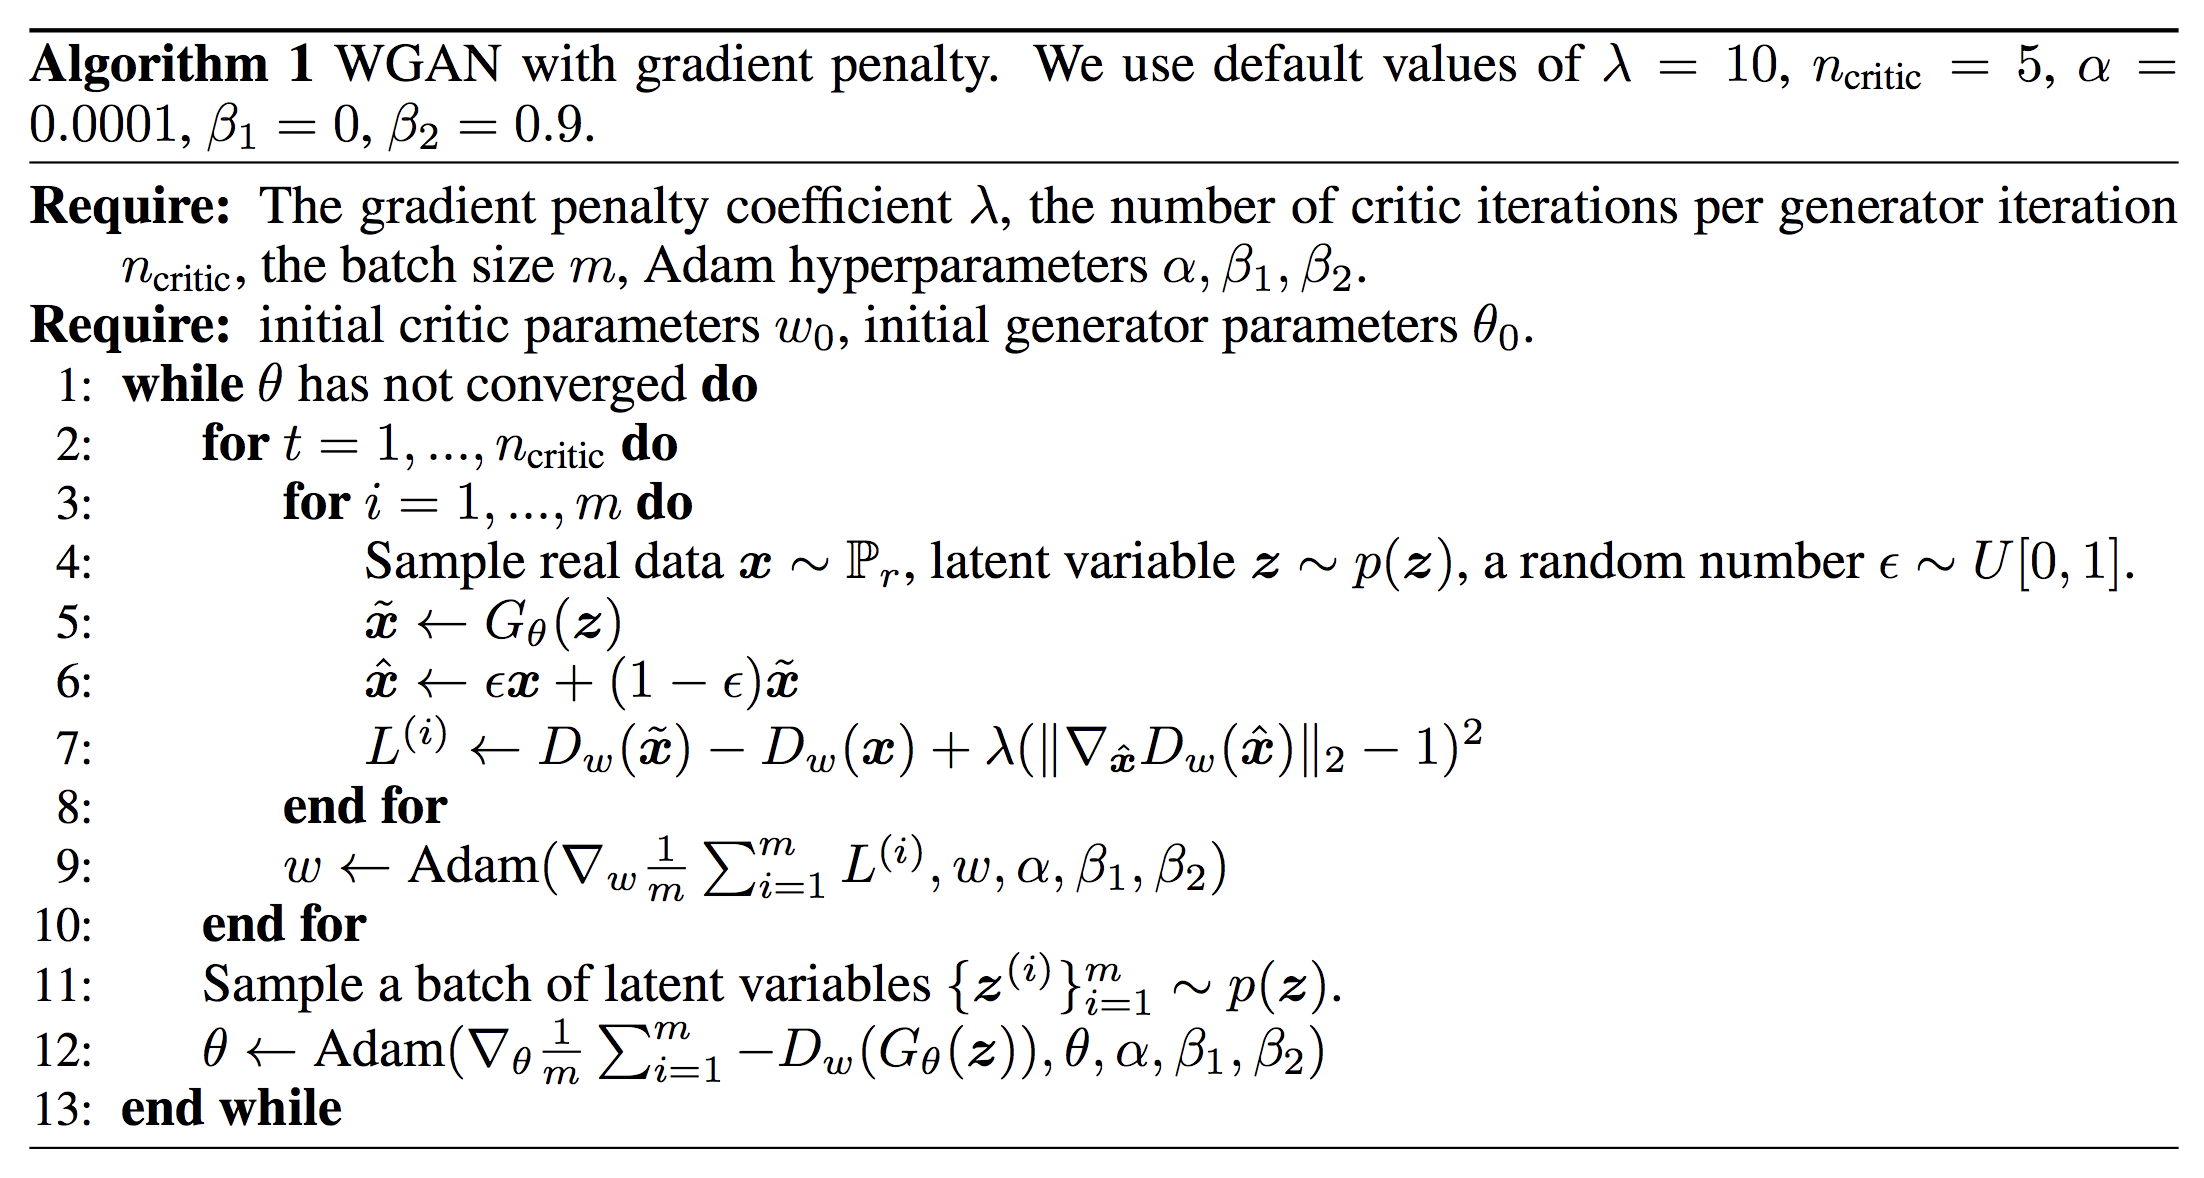
\includegraphics[height=0.8\textheight, width=1.05\textwidth, keepaspectratio]{images/gan/wgan-gp/slide_86_1_img.png}
        \caption*{[Gulrajani et al 2017]}
    \end{figure}
\end{frame}

\begin{frame}[allowframebreaks]{WGAN-GP: BatchNorm}
    \begin{figure}
        \centering
        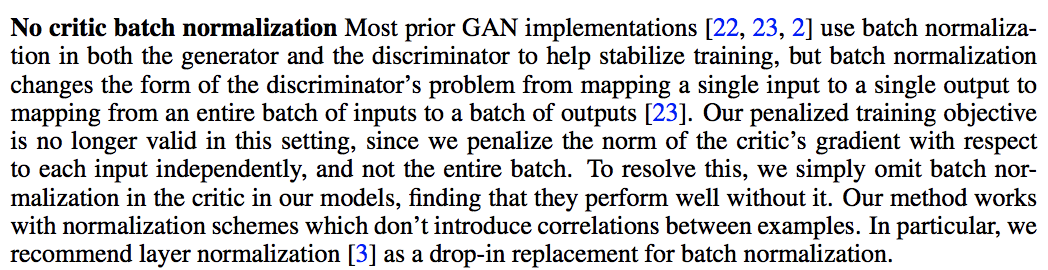
\includegraphics[height=0.8\textheight, width=1.05\textwidth, keepaspectratio]{images/gan/wgan-gp/slide_87_1_img.png}
        \caption*{[Gulrajani et al 2017]}
    \end{figure}
\end{frame}

\begin{frame}[allowframebreaks]{WGAN-GP: Robustness to architectures}
    \begin{figure}
        \centering
        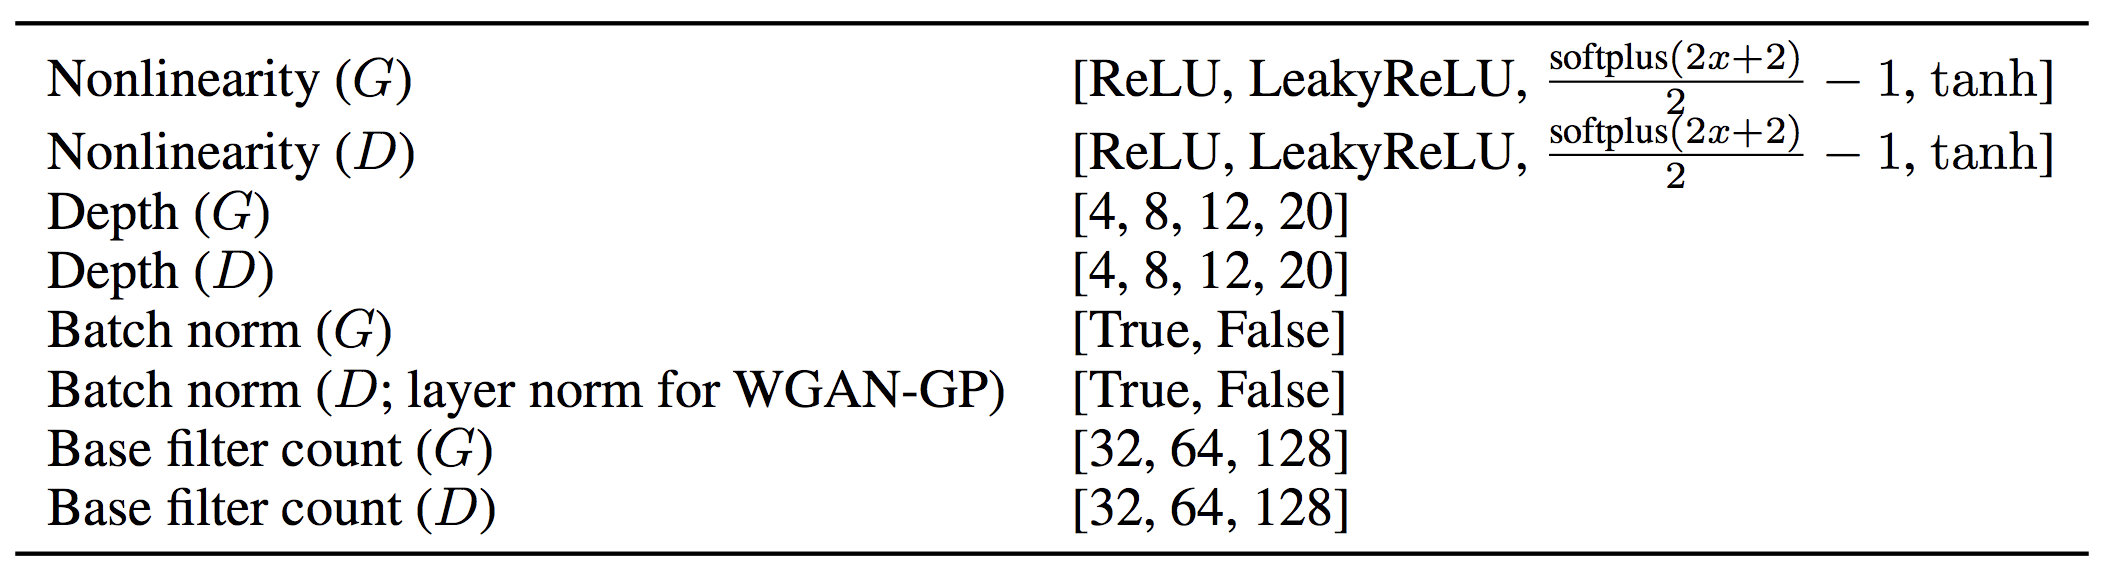
\includegraphics[height=0.8\textheight, width=1.05\textwidth, keepaspectratio]{images/gan/wgan-gp/slide_88_1_img.png}
    \end{figure}
    \begin{figure}
        \centering
        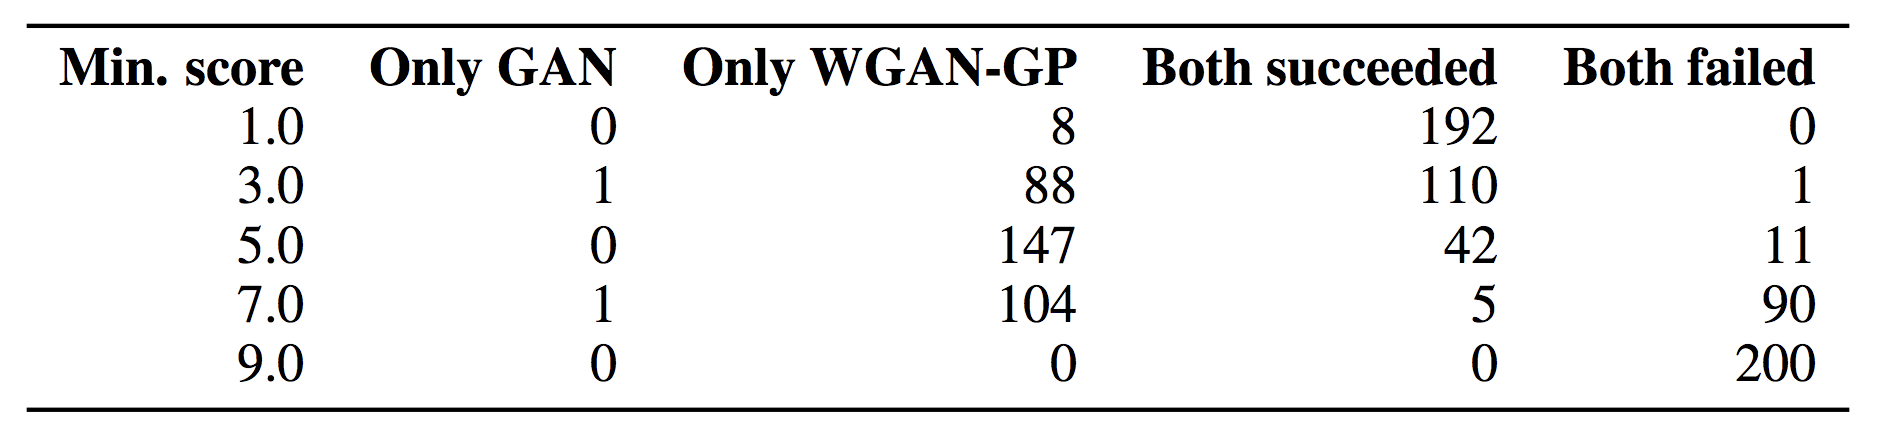
\includegraphics[height=0.8\textheight, width=1.05\textwidth, keepaspectratio]{images/gan/wgan-gp/slide_88_2_img.png}
        \caption*{[Gulrajani et al 2017]}
    \end{figure}

    \framebreak

    \begin{figure}
        \centering
        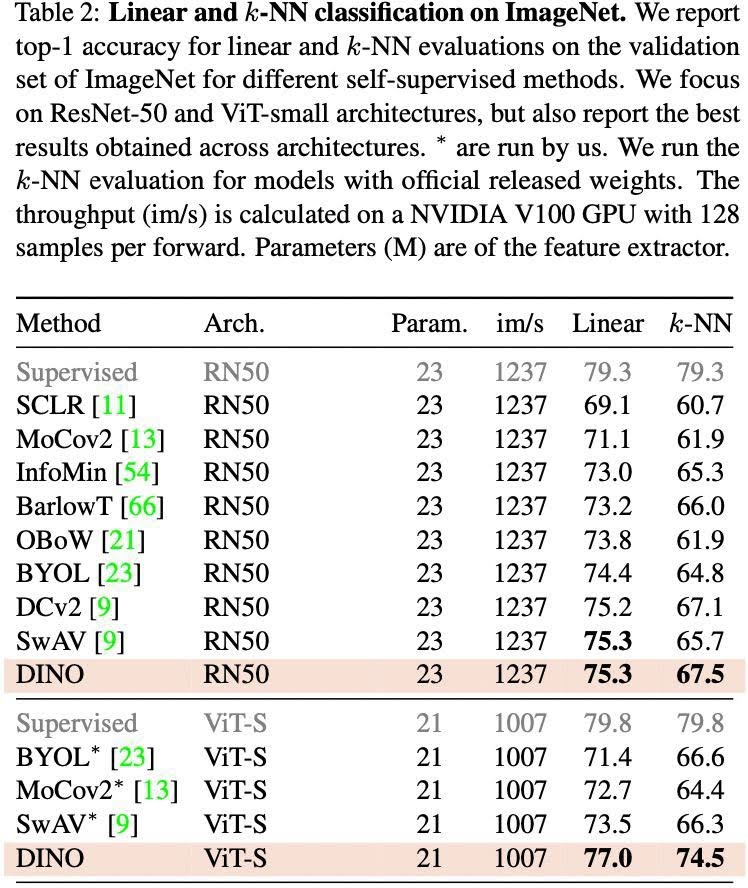
\includegraphics[height=0.85\textheight, width=1.05\textwidth, keepaspectratio]{images/gan/wgan-gp/slide_89_1_img.png}
        \caption*{[Gulrajani et al 2017]}
    \end{figure}
\end{frame}


\begin{frame}[allowframebreaks]{WGAN-GP: High quality samples}
    \begin{figure}
        \centering
        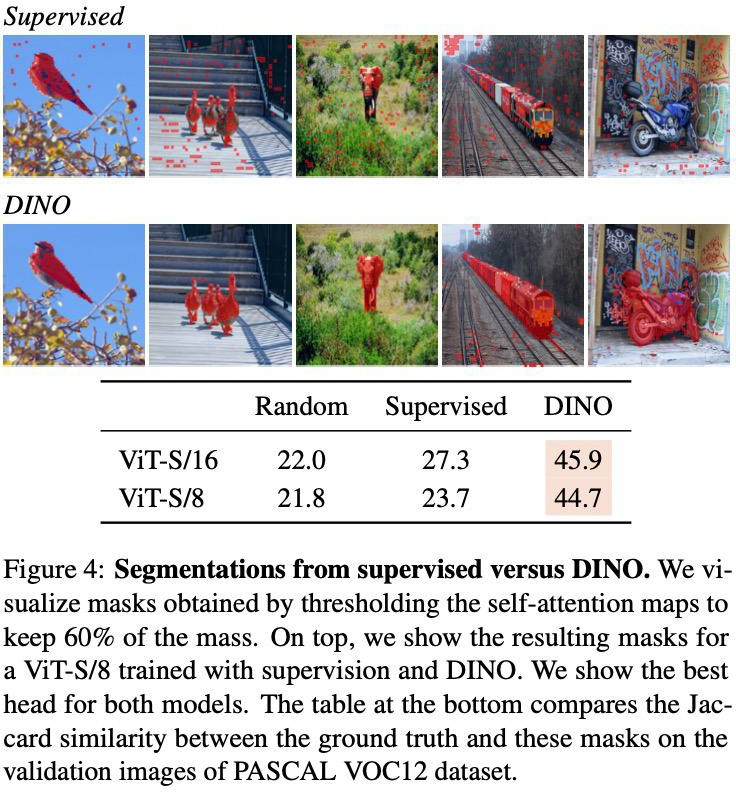
\includegraphics[height=0.8\textheight, width=1.05\textwidth, keepaspectratio]{images/gan/wgan-gp/slide_90_1_img.png}
        \caption*{[Gulrajani et al 2017]}
    \end{figure}

    \framebreak

    \begin{figure}
        \centering
        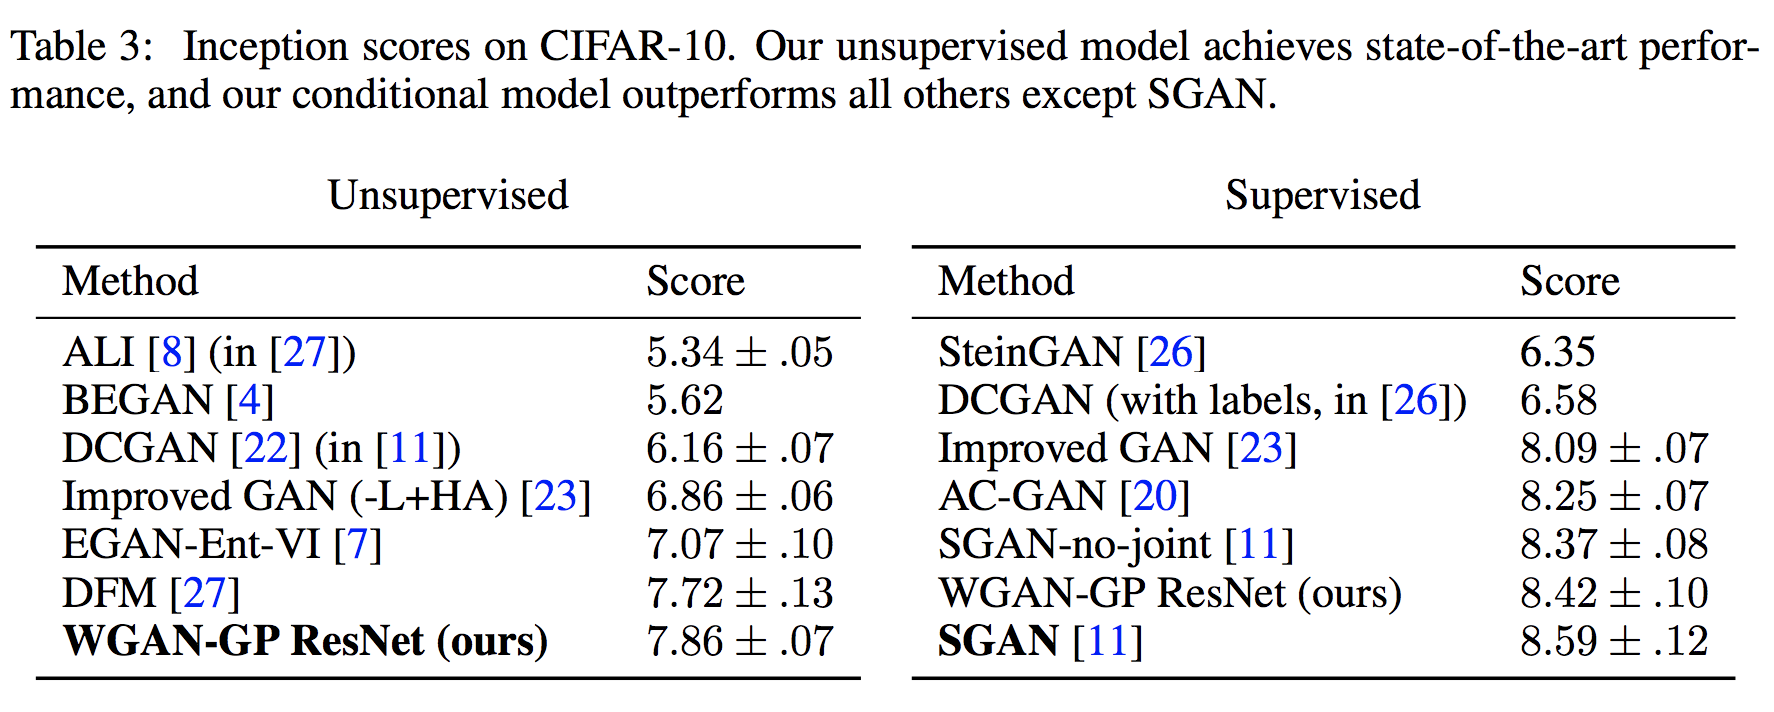
\includegraphics[height=0.8\textheight, width=1.05\textwidth, keepaspectratio]{images/gan/wgan-gp/slide_91_1_img.png}
        \caption*{[Gulrajani et al 2017]}
    \end{figure}
\end{frame}
\begin{frame}[allowframebreaks]{Conditional GAN}
\begin{itemize}
    \item In addition to random noise, a condition is added to the generator input. 
    \item The discriminator also receives this condition.
\end{itemize}
\begin{figure}
    \centering
    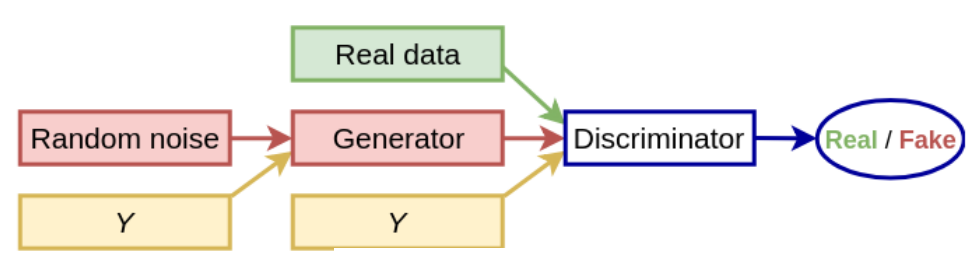
\includegraphics[height=0.8\textheight, width=\textwidth, keepaspectratio]{images/gan/cond_gan_1.png}
\end{figure}

\framebreak
\begin{itemize}
    \item Discriminator Loss:
    \begin{align*}
    \mathcal{L}^{(D)} \left( \theta^{(G)}, \theta^{(D)} \right) =\ & 
    - \mathbb{E}_{x \sim p_{data}} \left[ \log D(x|y) \right] \\
    & - \mathbb{E}_{z \sim p_z(z),\ y \sim p_{data}(y)} \left[ \log(1 - D(G(z|y))) \right]
    \end{align*}
    \item Generator Loss:
    $$
    \mathcal{L}^{(G)} \left( \theta^{(G)}, \theta^{(D)} \right) = - \mathbb{E}_z \left[ \log D(G(z|y)) \right]
    $$
\end{itemize}

\framebreak
\begin{figure}
    \centering
    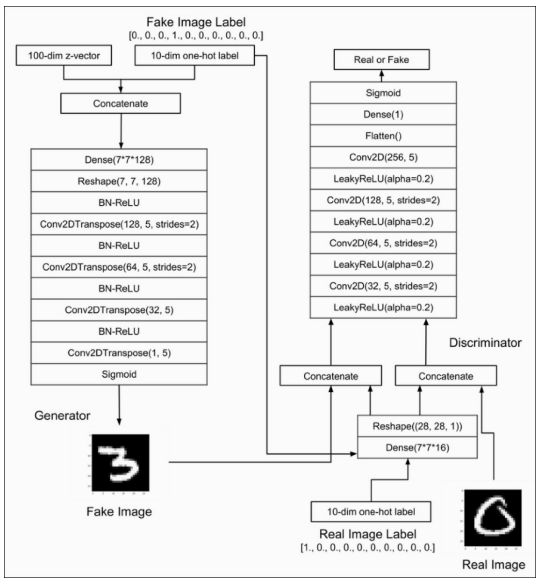
\includegraphics[height=0.8\textheight, width=\textwidth, keepaspectratio]{images/gan/cond_gan_2.png}
    \caption{A conditional GAN architecture for the MNIST digits dataset.}
\end{figure}

\end{frame}

\begin{frame}[allowframebreaks]{Condional GAN - Image to Image}

\begin{figure}
    \centering
    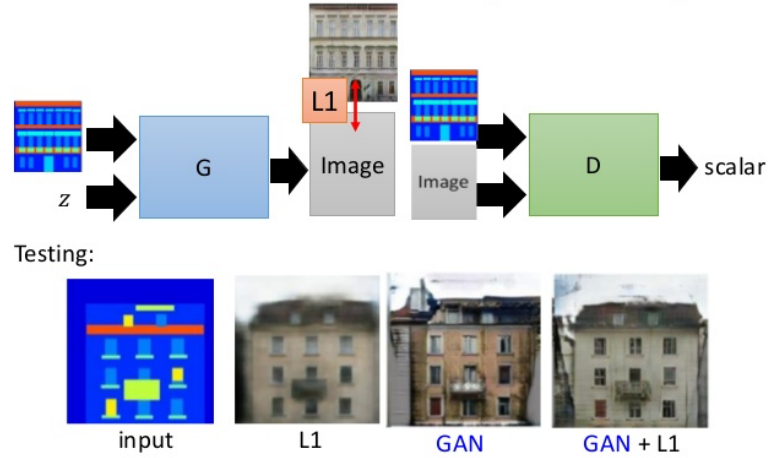
\includegraphics[height=0.75\textheight, width=\textwidth, keepaspectratio]{images/gan/cond_gan_3.png}
    \caption{Using L1 loss in addition in GAN loss can help in image to image translation}
\end{figure}

\framebreak

\begin{figure}
    \centering
    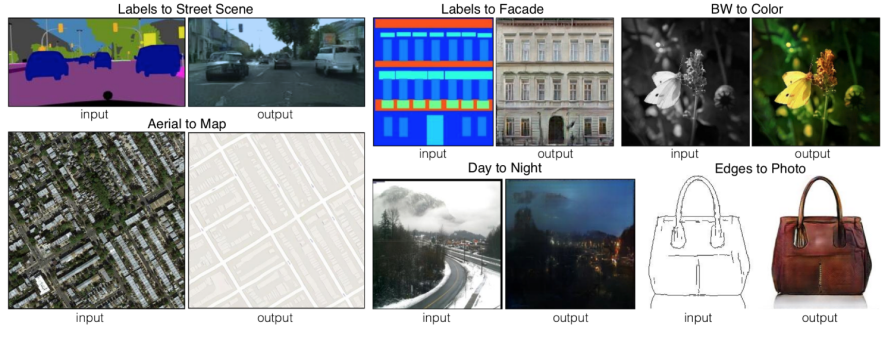
\includegraphics[height=0.8\textheight, width=\textwidth, keepaspectratio]{images/gan/cond_gan_4.png}
    \caption{Image to Image translation with condional GANs}
\end{figure}
    
\end{frame}
\begin{frame}[allowframebreaks]{Cycle GANs}

\begin{itemize}
    \item Unpaired Image-to-Image Translation using Cycle-Consistent Adversarial Networks, Efros, ICC7 2017
    
\end{itemize}
\begin{figure}
    \centering
    \includegraphics[height=0.7\textheight, width=\textwidth, keepaspectratio]{images/gan/cycle_gan_1.png}
\end{figure}
\framebreak
$$C_{horse \rightarrow zebra} = horse \rightarrow G_{horse \rightarrow zebra} \rightarrow \hat{zebra} \rightarrow [D_{zebra}, G_{zebra \rightarrow horse}] \rightarrow \hat{horse}$$
\begin{figure}
    \centering
    \includegraphics[height=0.7\textheight, width=\textwidth, keepaspectratio]{images/gan/cycle_gan_2.png}
\end{figure}

\framebreak
$$C_{zebra \rightarrow horse} = zebra \rightarrow G_{zebra \rightarrow horse} \rightarrow \hat{horse} \rightarrow [D_{horse}, G_{horse \rightarrow zebra}] \rightarrow \hat{zebra}$$
\begin{figure}
    \centering
    \includegraphics[height=0.7\textheight, width=\textwidth, keepaspectratio]{images/gan/cycle_gan_3.png}
\end{figure}

\framebreak
\begin{figure}
    \centering
    \includegraphics[height=0.7\textheight, width=\textwidth, keepaspectratio]{images/gan/cycle_gan_3.png}
\end{figure}

\framebreak
\begin{figure}
    \centering
    \includegraphics[height=0.9\textheight, width=\textwidth, keepaspectratio]{images/gan/cycle_gan_4.png}
\end{figure}

\framebreak
\begin{figure}
    \centering
    \includegraphics[height=0.9\textheight, width=\textwidth, keepaspectratio]{images/gan/cycle_gan_5.png}
\end{figure}

\framebreak
\begin{figure}
    \centering
    \includegraphics[height=0.9\textheight, width=\textwidth, keepaspectratio]{images/gan/cycle_gan_6.png}
    \caption{Image to Image translation with Cycle GANs}
\end{figure}
\end{frame}
\subsection{Style GANs}
\begin{frame}{}
    \LARGE GAN Variant: \\[1.5ex] \textbf{Style GANs}
\end{frame}

\begin{frame}[allowframebreaks]{Style GANs}
\begin{itemize}
    \item Goal: Better disentanglement of features in latent space (\textbf{W} space)
\end{itemize}
    \begin{figure}
    \centering
    \includegraphics[height=0.9\textheight, width=\textwidth, keepaspectratio]{images/gan/stylegan_2.png}
\end{figure}

\footnotetext{https://www.cs.unc.edu/~ronisen/teaching/fall_2022/pdf_lectures/lecture6_gan2.pdf}
\end{frame}
\begin{frame}[allowframebreaks]{Style GANs}
\begin{figure}
    \centering
    \includegraphics[height=0.9\textheight, width=\textwidth, keepaspectratio]{images/gan/stylegan_1.png}
\end{figure}
\footnotetext{https://arxiv.org/pdf/1812.04948}
\end{frame}
\begin{frame}[allowframebreaks]{Style GANs}

\begin{itemize}
    \item \textbf{A} = learned affine transformation block for AdaIN (predicts y)
    \item \textbf{Ada}ptive \textbf{I}stance \textbf{N}ormalization (very effective in controlling styles)
    $$\text{AdaIN}(x_i,y) = y_{s,i}\frac{x_i - u(x_i}{\sigma(x_i)} + y_{b,i}$$
    \item \textbf{B} = learned per-channel scaling factor for noise input.

\end{itemize}

\end{frame}

\begin{frame}[allowframebreaks]{Which Latent space to choose for embedding and editing?}
\begin{itemize}
    \item \textbf{Z} : 512 dimensional latent space (not good)
    \item \textbf{W} : 512 dimensional latent space (better but not perfect)
    \item \textbf{W+} : 18x512 dimensional latent space (after affine transformation \textbf{A} has been applied)
    \item \textbf{W} is better for editing.
    \item \textbf{W+} is better for reconstruction or embedding of real images.
\end{itemize}

\end{frame}

\begin{frame}[allowframebreaks]{Style GANs - Results}
\begin{figure}
    \centering
    \includegraphics[height=0.9\textheight, width=\textwidth, keepaspectratio]{images/gan/stylegan_3.png}
\end{figure}
\footnotetext{https://arxiv.org/pdf/1812.04948}
\end{frame}
\begin{frame}{}
    \LARGE GAN Variant: \\[1.5ex] \textbf{Wasserstein GANs (WGANs)}
\end{frame}

\begin{frame}[allowframebreaks]{Wasserstein GAN}
\begin{itemize}
    \item Wasserstein GAN uses wasserstein distance instead of crossentropy loss.
    \item Wasserstein distance that has a smoother gradient everywhere.
        \begin{figure}
            \centering
            \includegraphics[height=0.6\textheight, width=\textwidth, keepaspectratio]{images/gan/wgan_1.png}
        \end{figure}
\end{itemize}
    
\end{frame}

\begin{frame}{Wasserstein Distance}
\begin{itemize}
    \item Intuitively, it is the shovels of earth moved to make two distributions look alike.
    \begin{figure}
        \centering
        \includegraphics[height=0.6\textheight, width=\textwidth, keepaspectratio]{images/gan/wgan_2.png}
        \caption*{Step by Step plan of moving dirt between piles $P$ and $Q$ to make them match}
    \end{figure}
    
\end{itemize}
    
\end{frame}

\begin{frame}[allowframebreaks]{WGAN}
\begin{figure}
    \centering
    \includegraphics[height=0.9\textheight, width=\textwidth, keepaspectratio]{images/gan/wgan_3.png}
\end{figure}

\framebreak
\begin{figure}
    \centering
    \includegraphics[height=0.9\textheight, width=\textwidth, keepaspectratio]{images/gan/wgan_4.png}
\end{figure}

\framebreak
\begin{figure}
    \centering
    \includegraphics[height=0.8\textheight, width=\textwidth, keepaspectratio]{images/gan/wgan_5.png}
    \caption*{WGAN generation results on bedroom images}
\end{figure}

\end{frame}

\begin{frame}[allowframebreaks]{WGAN-GP: Gradient Penalty for Lipschitzness}
\begin{figure}
    \centering
    \includegraphics[height=0.8\textheight, width=\textwidth, keepaspectratio]{images/gan/wgan-gp/slide_84_1_img.png}
    \caption*{[Gulrajani et al 2017]}
\end{figure}

\framebreak
\begin{columns}
    \column{0.6\textwidth}
    \begin{figure}
        \centering
        \includegraphics[height=0.8\textheight, width=\textwidth, keepaspectratio]{images/gan/wgan-gp/slide_85_3_img.png}
    \end{figure}
    \begin{figure}
        \centering
        \includegraphics[height=0.1\textheight, width=\textwidth, keepaspectratio]{images/gan/wgan-gp/slide_85_4_img.png}
    \end{figure}
    \column{0.5\textwidth}
    \begin{figure}
        \centering
        \includegraphics[height=0.8\textheight, width=1.05\textwidth, keepaspectratio]{images/gan/wgan-gp/slide_85_2_img.png}
    \end{figure}
    \begin{figure}
        \centering
        \includegraphics[height=0.8\textheight, width=1.05\textwidth, keepaspectratio]{images/gan/wgan-gp/slide_85_1_img.png}
    \end{figure}
\end{columns}
\end{frame}

\begin{frame}[allowframebreaks]{WGAN-GP: Pseudocode}
    \begin{figure}
        \centering
        \includegraphics[height=0.8\textheight, width=1.05\textwidth, keepaspectratio]{images/gan/wgan-gp/slide_86_1_img.png}
        \caption*{[Gulrajani et al 2017]}
    \end{figure}
\end{frame}

\begin{frame}[allowframebreaks]{WGAN-GP: BatchNorm}
    \begin{figure}
        \centering
        \includegraphics[height=0.8\textheight, width=1.05\textwidth, keepaspectratio]{images/gan/wgan-gp/slide_87_1_img.png}
        \caption*{[Gulrajani et al 2017]}
    \end{figure}
\end{frame}

\begin{frame}[allowframebreaks]{WGAN-GP: Robustness to architectures}
    \begin{figure}
        \centering
        \includegraphics[height=0.8\textheight, width=1.05\textwidth, keepaspectratio]{images/gan/wgan-gp/slide_88_1_img.png}
    \end{figure}
    \begin{figure}
        \centering
        \includegraphics[height=0.8\textheight, width=1.05\textwidth, keepaspectratio]{images/gan/wgan-gp/slide_88_2_img.png}
        \caption*{[Gulrajani et al 2017]}
    \end{figure}

    \framebreak

    \begin{figure}
        \centering
        \includegraphics[height=0.85\textheight, width=1.05\textwidth, keepaspectratio]{images/gan/wgan-gp/slide_89_1_img.png}
        \caption*{[Gulrajani et al 2017]}
    \end{figure}
\end{frame}


\begin{frame}[allowframebreaks]{WGAN-GP: High quality samples}
    \begin{figure}
        \centering
        \includegraphics[height=0.8\textheight, width=1.05\textwidth, keepaspectratio]{images/gan/wgan-gp/slide_90_1_img.png}
        \caption*{[Gulrajani et al 2017]}
    \end{figure}

    \framebreak

    \begin{figure}
        \centering
        \includegraphics[height=0.8\textheight, width=1.05\textwidth, keepaspectratio]{images/gan/wgan-gp/slide_91_1_img.png}
        \caption*{[Gulrajani et al 2017]}
    \end{figure}
\end{frame}
\begin{frame}[allowframebreaks]{Conditional GAN}
\begin{itemize}
    \item In addition to random noise, a condition is added to the generator input. 
    \item The discriminator also receives this condition.
\end{itemize}
\begin{figure}
    \centering
    \includegraphics[height=0.8\textheight, width=\textwidth, keepaspectratio]{images/gan/cond_gan_1.png}
\end{figure}

\framebreak
\begin{itemize}
    \item Discriminator Loss:
    \begin{align*}
    \mathcal{L}^{(D)} \left( \theta^{(G)}, \theta^{(D)} \right) =\ & 
    - \mathbb{E}_{x \sim p_{data}} \left[ \log D(x|y) \right] \\
    & - \mathbb{E}_{z \sim p_z(z),\ y \sim p_{data}(y)} \left[ \log(1 - D(G(z|y))) \right]
    \end{align*}
    \item Generator Loss:
    $$
    \mathcal{L}^{(G)} \left( \theta^{(G)}, \theta^{(D)} \right) = - \mathbb{E}_z \left[ \log D(G(z|y)) \right]
    $$
\end{itemize}

\framebreak
\begin{figure}
    \centering
    \includegraphics[height=0.8\textheight, width=\textwidth, keepaspectratio]{images/gan/cond_gan_2.png}
    \caption{A conditional GAN architecture for the MNIST digits dataset.}
\end{figure}

\end{frame}

\begin{frame}[allowframebreaks]{Condional GAN - Image to Image}

\begin{figure}
    \centering
    \includegraphics[height=0.75\textheight, width=\textwidth, keepaspectratio]{images/gan/cond_gan_3.png}
    \caption{Using L1 loss in addition in GAN loss can help in image to image translation}
\end{figure}

\framebreak

\begin{figure}
    \centering
    \includegraphics[height=0.8\textheight, width=\textwidth, keepaspectratio]{images/gan/cond_gan_4.png}
    \caption{Image to Image translation with condional GANs}
\end{figure}
    
\end{frame}
\begin{frame}[allowframebreaks]{Cycle GANs}

\begin{itemize}
    \item Unpaired Image-to-Image Translation using Cycle-Consistent Adversarial Networks, Efros, ICC7 2017
    
\end{itemize}
\begin{figure}
    \centering
    \includegraphics[height=0.7\textheight, width=\textwidth, keepaspectratio]{images/gan/cycle_gan_1.png}
\end{figure}
\framebreak
$$C_{horse \rightarrow zebra} = horse \rightarrow G_{horse \rightarrow zebra} \rightarrow \hat{zebra} \rightarrow [D_{zebra}, G_{zebra \rightarrow horse}] \rightarrow \hat{horse}$$
\begin{figure}
    \centering
    \includegraphics[height=0.7\textheight, width=\textwidth, keepaspectratio]{images/gan/cycle_gan_2.png}
\end{figure}

\framebreak
$$C_{zebra \rightarrow horse} = zebra \rightarrow G_{zebra \rightarrow horse} \rightarrow \hat{horse} \rightarrow [D_{horse}, G_{horse \rightarrow zebra}] \rightarrow \hat{zebra}$$
\begin{figure}
    \centering
    \includegraphics[height=0.7\textheight, width=\textwidth, keepaspectratio]{images/gan/cycle_gan_3.png}
\end{figure}

\framebreak
\begin{figure}
    \centering
    \includegraphics[height=0.7\textheight, width=\textwidth, keepaspectratio]{images/gan/cycle_gan_3.png}
\end{figure}

\framebreak
\begin{figure}
    \centering
    \includegraphics[height=0.9\textheight, width=\textwidth, keepaspectratio]{images/gan/cycle_gan_4.png}
\end{figure}

\framebreak
\begin{figure}
    \centering
    \includegraphics[height=0.9\textheight, width=\textwidth, keepaspectratio]{images/gan/cycle_gan_5.png}
\end{figure}

\framebreak
\begin{figure}
    \centering
    \includegraphics[height=0.9\textheight, width=\textwidth, keepaspectratio]{images/gan/cycle_gan_6.png}
    \caption{Image to Image translation with Cycle GANs}
\end{figure}
\end{frame}
\subsection{Style GANs}
\begin{frame}{}
    \LARGE GAN Variant: \\[1.5ex] \textbf{Style GANs}
\end{frame}

\begin{frame}[allowframebreaks]{Style GANs}
\begin{itemize}
    \item Goal: Better disentanglement of features in latent space (\textbf{W} space)
\end{itemize}
    \begin{figure}
    \centering
    \includegraphics[height=0.9\textheight, width=\textwidth, keepaspectratio]{images/gan/stylegan_2.png}
\end{figure}

\footnotetext{https://www.cs.unc.edu/~ronisen/teaching/fall_2022/pdf_lectures/lecture6_gan2.pdf}
\end{frame}
\begin{frame}[allowframebreaks]{Style GANs}
\begin{figure}
    \centering
    \includegraphics[height=0.9\textheight, width=\textwidth, keepaspectratio]{images/gan/stylegan_1.png}
\end{figure}
\footnotetext{https://arxiv.org/pdf/1812.04948}
\end{frame}
\begin{frame}[allowframebreaks]{Style GANs}

\begin{itemize}
    \item \textbf{A} = learned affine transformation block for AdaIN (predicts y)
    \item \textbf{Ada}ptive \textbf{I}stance \textbf{N}ormalization (very effective in controlling styles)
    $$\text{AdaIN}(x_i,y) = y_{s,i}\frac{x_i - u(x_i}{\sigma(x_i)} + y_{b,i}$$
    \item \textbf{B} = learned per-channel scaling factor for noise input.

\end{itemize}

\end{frame}

\begin{frame}[allowframebreaks]{Which Latent space to choose for embedding and editing?}
\begin{itemize}
    \item \textbf{Z} : 512 dimensional latent space (not good)
    \item \textbf{W} : 512 dimensional latent space (better but not perfect)
    \item \textbf{W+} : 18x512 dimensional latent space (after affine transformation \textbf{A} has been applied)
    \item \textbf{W} is better for editing.
    \item \textbf{W+} is better for reconstruction or embedding of real images.
\end{itemize}

\end{frame}

\begin{frame}[allowframebreaks]{Style GANs - Results}
\begin{figure}
    \centering
    \includegraphics[height=0.9\textheight, width=\textwidth, keepaspectratio]{images/gan/stylegan_3.png}
\end{figure}
\footnotetext{https://arxiv.org/pdf/1812.04948}
\end{frame}
\begin{frame}{}
    \LARGE GANs: \textbf{Latent space Interpolation}
\end{frame}

\begin{frame}[allowframebreaks]{Latent space Interpolation}
\begin{figure}
    \centering
    \includegraphics[height=0.9\textheight, width=\textwidth, keepaspectratio]{images/gan/gan_latent.png}
    \caption*{Latent space interploation with GANs}
\end{figure}
\framebreak
\centering
Latent space interpolation with StyleGAN\\
\centering
(Demo by Xander Steenburgge)\\

\vspace{\baselineskip}

\centering
\href{https://colab.research.google.com/drive/1mH70YxGNlnEaSOn0J8Lsgkl-QOvsIb3M#scrollTo=uEhxBvAR-7y3}{https://colab.research.google.com/drive/1mH70YxGNlnEaSOn0J8Lsgkl-QOvsIb3M#scrollTo=uEhxBvAR-7y3}
\end{frame}
\section{More Results}
\begin{frame}{}
    \LARGE GANs: \textbf{More Results}
\end{frame}

\begin{frame}[allowframebreaks]{Some more GAN results}
\begin{figure}
    \centering
    \includegraphics[height=0.8\textheight, width=\textwidth, keepaspectratio]{images/gan/gan_results_4.png}
    \caption*{Image Inpainting. https://www.nvidia.com/en-us/research/ai-demos/}
\end{figure}

\framebreak

\begin{figure}
    \centering
    \includegraphics[height=0.8\textheight, width=\textwidth, keepaspectratio]{images/gan/gan_results_5.png}
    \caption*{Text to Image Synthesis with GANs}
\end{figure}

\framebreak

\begin{figure}
    \centering
    \includegraphics[height=0.8\textheight, width=\textwidth, keepaspectratio]{images/gan/gan_results_6.png}
    \caption*{Living Portraits with GANs}
\end{figure}

\begin{figure}
    \centering
    \includegraphics[height=0.8\textheight, width=\textwidth, keepaspectratio]{images/gan/gan_results_7.png}
    \caption*{Image to Image translation in multiple domains with StyleGAN (Choi et al.)}
\end{figure}
\end{frame}
\begin{frame}[allowframebreaks]{Summary}
\begin{itemize}
    \item \textbf{SimCLR:}
    \begin{itemize}
        \item Simple framework for contrastive learning.
        \item Uses data augmentation and contrastive loss.
    \end{itemize}
    \item \textbf{BYOL:}
    \begin{itemize}
        \item Self-supervised approach without negative pairs.
        \item Uses two networks: online and target.
    \end{itemize}
    \item \textbf{DINO:}
    \begin{itemize}
        \item Self-distillation method without labels.
        \item Uses teacher-student networks and knowledge distillation.
    \end{itemize}

    \framebreak

    \item \textbf{DINOv2:}
    \begin{itemize}
        \item Improved version of DINO.
        \item Enhanced training strategies and architectures.
        \item Better performance and scalability.
    \end{itemize}
    \item \textbf{iBOT:}
    \begin{itemize}
        \item Combines contrastive learning with masked image modeling.
        \item Uses BERT-style pretraining and vision transformers.
    \end{itemize}
\end{itemize}
\end{frame}
\begin{frame}[allowframebreaks]{Appendix}
\begin{block}{GANs: Definition and Core Components:}
    \begin{itemize}
        \item \textbf{Definition}: Generative Adversarial Networks (GANs) consist of two neural networks trained in opposition to each other.
        \item \textbf{Core Components:}
        \begin{itemize}
            \item \textbf{Generator (G):} Takes random noise (latent vector) and produces fake data samples.
            \item \textbf{Discriminator (D):} Receives real or fake data and predicts whether the input is real.
        \end{itemize}
        \item \textbf{Mathematical Formulation:}
    \end{itemize}
    \begin{equation*}
        \min_G \max_D \; \mathbb{E}_{x \sim p_{\text{data}}} [\log D(x)] + \mathbb{E}_{z \sim p_z} [\log(1 - D(G(z)))]
    \end{equation*}
    \begin{itemize}
        \item[] Where:
        \begin{itemize}
            \item $x$: Real data sample
            \item $z$: Noise vector sampled from prior $p_z$
            \item $G(z)$: Generated sample
        \end{itemize}
    \end{itemize}
\end{block}


\end{frame}

\begin{frame}[plain]
  \frametitle{Credits}
  \begin{center}
    \textbf{Credits} \\[1.5em]

    \Large Dr. Prashant Aparajeya \\[0.5em]
    {\normalsize Computer Vision Scientist | Director(AISimply Ltd)} \\[0.5em]
    \footnotesize \href{mailto:p.aparajeya@aisimply.uk}{p.aparajeya@aisimply.uk} \\[2em]

    {\footnotesize This project benefited from external collaboration, and we acknowledge their contribution with gratitude.}
  \end{center}
\end{frame}


\end{document} 